\documentclass[11pt]{article}

\usepackage[a4paper,margin=27mm,headheight=14pt]{geometry}
\usepackage[T1]{fontenc}
\usepackage[utf8]{inputenc}
\usepackage{lmodern}
\usepackage{microtype}
\usepackage{amsmath,amssymb,amsthm,mathtools,bm}
\allowdisplaybreaks
\usepackage{booktabs,longtable,array,tabularx}
\usepackage{enumitem}
\usepackage{xcolor}
\usepackage{hyperref}
\usepackage[nameinlink,capitalise,noabbrev]{cleveref}
\usepackage{tikz}
\usepackage{pgfplots}
\pgfplotsset{compat=1.18}
\usepackage{listings}
\usepackage{fancyhdr}
\usepackage{caption}
\usepackage{subcaption}

\hypersetup{
  pdftitle={The Fabius Function and Rvachev's Up Function},
  pdfauthor={OpenAI, based on the formal development by Vladimir Reshetnikov},
  colorlinks=true,
  linkcolor=blue!55!black,
  citecolor=green!35!black,
  urlcolor=blue!60!black
}

\pagestyle{fancy}
\fancyhf{}
\fancyhead[L]{The Fabius function and Rvachev's up function}
\fancyhead[R]{\thepage}
\renewcommand{\headrulewidth}{0.3pt}

\numberwithin{equation}{section}
\setcounter{tocdepth}{2}
\setcounter{secnumdepth}{3}
\setlist{itemsep=2pt,topsep=5pt}

\newtheorem{theorem}{Theorem}[section]
\newtheorem{proposition}[theorem]{Proposition}
\newtheorem{lemma}[theorem]{Lemma}
\newtheorem{corollary}[theorem]{Corollary}
\newtheorem{claim}[theorem]{Claim}
\theoremstyle{definition}
\newtheorem{definition}[theorem]{Definition}
\newtheorem{algorithm}[theorem]{Algorithm}
\newtheorem{example}[theorem]{Example}
\theoremstyle{remark}
\newtheorem{remark}[theorem]{Remark}
\newtheorem{warning}[theorem]{Warning}

\DeclareMathOperator{\supp}{supp}
\DeclareMathOperator{\lcm}{lcm}
\DeclareMathOperator{\wt}{wt}
\DeclareMathOperator{\den}{den}
\DeclareMathOperator{\Res}{Res}
\DeclareMathOperator{\erf}{erf}
\DeclareMathOperator{\sgn}{sgn}
\newcommand{\R}{\mathbb R}
\newcommand{\Q}{\mathbb Q}
\newcommand{\Z}{\mathbb Z}
\newcommand{\N}{\mathbb N}
\newcommand{\C}{\mathbb C}
\newcommand{\F}{F}
\newcommand{\GF}{\mathcal F}
\newcommand{\upf}{\operatorname{up}}
\newcommand{\eps}{\varepsilon}
\newcommand{\sinc}{\operatorname{sinc}}
\newcommand{\dd}{\,\mathrm d}
\newcommand{\e}{\mathrm e}
\newcommand{\ii}{\mathrm i}
\newcommand{\Oh}{\mathrm O}
\newcommand{\littleoh}{\mathrm o}
\newcommand{\GaussBinom}[3]{\genfrac{[}{]}{0pt}{}{#1}{#2}_{#3}}
\newcommand{\abs}[1]{\left|#1\right|}
\newcommand{\norm}[1]{\left\lVert#1\right\rVert}
\newcommand{\set}[1]{\left\{#1\right\}}
\newcommand{\floor}[1]{\left\lfloor#1\right\rfloor}
\newcommand{\ceil}[1]{\left\lceil#1\right\rceil}
\newcommand{\angles}[1]{\left\langle#1\right\rangle}
\newcommand{\binomtwo}[1]{\binom{#1}{2}}

\title{\textbf{The Fabius Function and Rvachev's Up Function}\\[0.5em]
\large Self-similarity, probability, exact dyadic arithmetic, and the corrected small-argument asymptotic}
\author{A human-readable synthesis of the Lean development in the \texttt{ProveIt} repository}
\date{24 August 2026}

\begin{document}
\maketitle

\begin{abstract}
The Fabius function is one of the most striking elementary-looking objects in real analysis: it is a strictly increasing $C^\infty$ distribution function on $[0,1]$, flat at both endpoints, symmetric about $(1/2,1/2)$, and governed by a dyadic differential equation.  Its close relative, Rvachev's compactly supported \emph{up function}, is an even positive bump on $[-1,1]$ whose derivative is the difference of two rescaled translates of itself.  The two functions admit descriptions by infinite convolutions, random series, Fourier products, Poisson summation, moments, entire generating functions, terminating Taylor formulas at dyadic points, and exact rational algorithms.

This article gives a self-contained mathematical exposition of the substantive results formalized in Vladimir Reshetnikov's Lean development \cite{ProveIt}, which verifies the two papers of Arias de Reyna \cite{Arias05442,Arias06487} and extends them in several directions.  Particular attention is devoted to two topics.  First, we prove exact formulas for values at arbitrary dyadic rationals, including a fast highest-bit recursion and a finite $q$-binomial/Thue--Morse identity valid for the signed global extension.  Second, we derive the corrected endpoint asymptotic.  The sharp expansion is naturally expressed in a lower-Lambert phase $\lambda$, contains a nonconstant one-periodic Gamma--zeta fluctuation, and possesses a complete expansion in inverse powers of $\lambda$.  Omitting that periodic term destroys the asserted sharp error estimate.

The exposition deliberately distinguishes the bounded cumulative-distribution function from the signed global continuation: both have often been denoted by $F$, but confusing them leads to false global identities.  We also record the minor corrections to the printed source formulas detected and certified by the formalization.  The aim is not to reproduce thousands of implementation lemmas, but to present the principal theorem families and their proof mechanisms in conventional mathematical language.
\end{abstract}

\tableofcontents
\newpage

\section{Orientation and conventions}

\subsection{Three versions of the same dyadic object}

There are three functions in this story, and it is important not to merge them prematurely.

\begin{definition}[The bounded Fabius function]
The \emph{bounded Fabius function} is the function $F:\R\to[0,1]$ characterized by
\begin{align}
 F(x)&=0 &&(x\le 0),\label{eq:F-left-clamp}\\
 F(x)&=1 &&(x\ge 1),\label{eq:F-right-clamp}\\
 F(x)+F(1-x)&=1 &&(0\le x\le1),\label{eq:F-symmetry}\\
 F'(x)&=2F(2x) &&(0\le x\le\tfrac12),\label{eq:F-diff}
\end{align}
and by the requirement $F\in C^\infty(\R)$.  The canonical existence and uniqueness theorem is proved in \cref{sec:existence}.
\end{definition}

Thus $F$ is a genuine cumulative distribution function.  On the right half of the unit interval, differentiating \eqref{eq:F-symmetry} gives the companion formula
\begin{equation}\label{eq:F-right-derivative}
 F'(x)=2\bigl(1-F(2x-1)\bigr),\qquad \tfrac12\le x\le1.
\end{equation}
The clamped function does \emph{not} satisfy $F'(x)=2F(2x)$ on all of $\R$.

\begin{definition}[The signed global extension]
Let $s_2(n)$ denote the sum of the binary digits of $n$, and put
\begin{equation}\label{eq:thue-morse-sign}
 \eps_n:=(-1)^{s_2(n)}\qquad(n\ge0).
\end{equation}
The \emph{signed global Fabius extension} is
\begin{equation}\label{eq:global-F-def}
 \GF(x):=\sum_{n=0}^{\infty}\eps_n\,\upf(x-2n-1).
\end{equation}
Because $\upf$ is supported on $[-1,1]$, the sum is locally finite.  It agrees with the bounded function on $[0,1]$, but outside that interval it oscillates and can be negative; for example, $\GF(3)=-1$.
\end{definition}

\begin{definition}[Rvachev's up function]
The \emph{up function} $\upf:\R\to\R$ is the unique $C^\infty$ function such that
\begin{equation}\label{eq:up-basic}
 \supp(\upf)=[-1,1],\qquad \upf>0\text{ on }(-1,1),\qquad \upf(0)=1,
\end{equation}
and
\begin{equation}\label{eq:up-differential}
 \upf'(x)=2\bigl(\upf(2x+1)-\upf(2x-1)\bigr)
 \qquad(x\in\R).
\end{equation}
\end{definition}

On the natural support interval, the three conventions are related by
\begin{equation}\label{eq:F-up-relations}
 \upf(t)=\GF(t+1)=
 \begin{cases}
   F(t+1),&-1\le t\le0,\\
   F(1-t),&0\le t\le1,
 \end{cases}
 \qquad
 F(x)=\upf(x-1)\quad(0\le x\le1).
\end{equation}
The last formula uses the evenness of $\upf$.  It explains the description of the two functions as twins: the left half of the bump is exactly the CDF, shifted by one unit, while the right half is its reflected survival function.

\begin{warning}[A notation trap]
Arias de Reyna's papers use the same letter $F$ for the unit-interval function and for a signed continuation.  Statements such as
\[
 \GF^{(k)}(x)=2^{\binom{k+1}{2}}\GF(2^kx)
\]
are global statements about $\GF$.  Their bounded counterparts must be restricted to points for which every scaled argument remains in $[0,1]$.  The Lean development makes this type distinction explicit, and we follow it throughout.
\end{warning}

\subsection{Historical remarks}

The infinite Fourier product underlying $\upf$ appeared in work of Jessen and Wintner in 1935 \cite{JessenWintner}.  Fabius used the associated distribution in 1966 to exhibit a nowhere analytic $C^\infty$ function \cite{Fabius1966}.  Rvachev developed the compactly supported function and related ``atomic functions'' as tools in approximation and numerical analysis \cite{Rvachev1990}.  A systematic account of the defining equation, probability interpretation, Fourier formulas, moment identities, Poisson summation, and dyadic rationality was written by Arias de Reyna in 1980 and later made available in English \cite{Arias05442}.  His arithmetic sequel \cite{Arias06487} studies the rational sequences hidden in the moments and answers an integrality question raised by Reshetnikov.

The formal development \cite{ProveIt} verifies all mathematically substantive statements in those two papers and adds, among other results, an executable exact evaluator, a Fourier--Legendre expansion, finite $q$-binomial/Thue--Morse formulas, and a corrected all-orders endpoint asymptotic.  This article is organized around the mathematics rather than the order of the source files.

\subsection{A first picture}

The following plot joins exact values on a grid of denominator $64$.  It is only a visual guide; all qualitative assertions will be proved independently.

\begin{figure}[htbp]
\centering
\begin{subfigure}{0.48\textwidth}
\centering
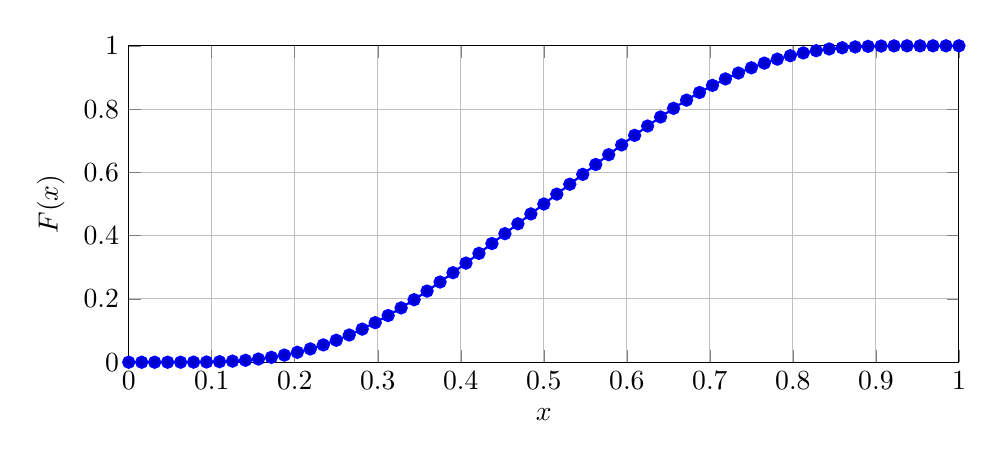
\begin{tikzpicture}
\begin{axis}[
 width=\linewidth,height=5.6cm,
 xmin=0,xmax=1,ymin=0,ymax=1,
 xlabel={$x$},ylabel={$F(x)$},
 grid=major,mark=none]
\addplot+[thick] coordinates {
(0.000000,0.000000000000)
(0.015625,0.000000002052)
(0.031250,0.000000572676)
(0.046875,0.000010468114)
(0.062500,0.000068962191)
(0.078125,0.000268172107)
(0.093750,0.000760121287)
(0.109375,0.001749676531)
(0.125000,0.003472222222)
(0.140625,0.006171330413)
(0.156250,0.010090573158)
(0.171875,0.015465334837)
(0.187500,0.022500482253)
(0.203125,0.031348038830)
(0.218750,0.042100121769)
(0.234375,0.054796004892)
(0.250000,0.069444444444)
(0.265625,0.086046004892)
(0.281250,0.104600121769)
(0.296875,0.125098038830)
(0.312500,0.147500482253)
(0.328125,0.171715334837)
(0.343750,0.197590573158)
(0.359375,0.224921330413)
(0.375000,0.253472222222)
(0.390625,0.282999676531)
(0.406250,0.313260121287)
(0.421875,0.344018172107)
(0.437500,0.375068962191)
(0.453125,0.406260468114)
(0.468750,0.437500572676)
(0.484375,0.468750002052)
(0.500000,0.500000000000)
(0.515625,0.531249997948)
(0.531250,0.562499427324)
(0.546875,0.593739531886)
(0.562500,0.624931037809)
(0.578125,0.655981827893)
(0.593750,0.686739878713)
(0.609375,0.717000323469)
(0.625000,0.746527777778)
(0.640625,0.775078669587)
(0.656250,0.802409426842)
(0.671875,0.828284665163)
(0.687500,0.852499517747)
(0.703125,0.874901961170)
(0.718750,0.895399878231)
(0.734375,0.913953995108)
(0.750000,0.930555555556)
(0.765625,0.945203995108)
(0.781250,0.957899878231)
(0.796875,0.968651961170)
(0.812500,0.977499517747)
(0.828125,0.984534665163)
(0.843750,0.989909426842)
(0.859375,0.993828669587)
(0.875000,0.996527777778)
(0.890625,0.998250323469)
(0.906250,0.999239878713)
(0.921875,0.999731827893)
(0.937500,0.999931037809)
(0.953125,0.999989531886)
(0.968750,0.999999427324)
(0.984375,0.999999997948)
(1.000000,1.000000000000)
};
\end{axis}
\end{tikzpicture}
\caption{The bounded Fabius CDF.}
\end{subfigure}\hfill
\begin{subfigure}{0.48\textwidth}
\centering
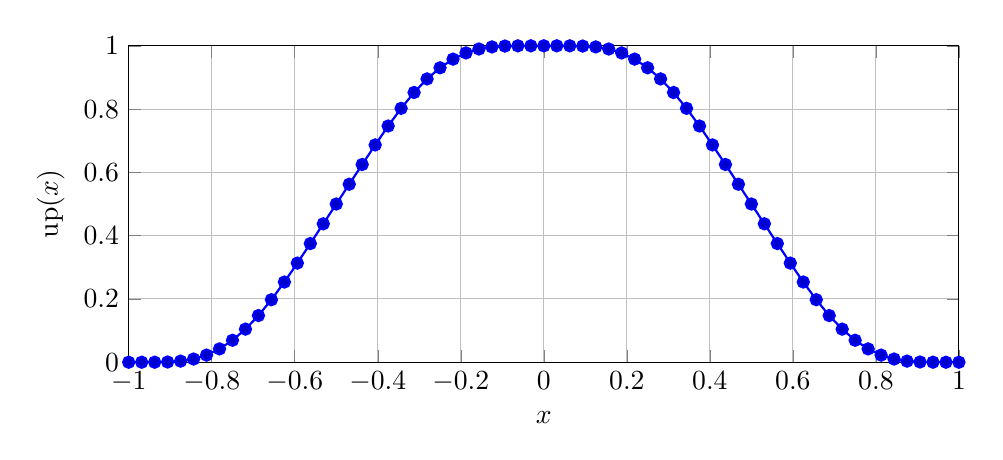
\begin{tikzpicture}
\begin{axis}[
 width=\linewidth,height=5.6cm,
 xmin=-1,xmax=1,ymin=0,ymax=1,
 xlabel={$x$},ylabel={$\upf(x)$},
 grid=major,mark=none]
\addplot+[thick] coordinates {
(-1.000000,0.000000000000)
(-0.968750,0.000000572676)
(-0.937500,0.000068962191)
(-0.906250,0.000760121287)
(-0.875000,0.003472222222)
(-0.843750,0.010090573158)
(-0.812500,0.022500482253)
(-0.781250,0.042100121769)
(-0.750000,0.069444444444)
(-0.718750,0.104600121769)
(-0.687500,0.147500482253)
(-0.656250,0.197590573158)
(-0.625000,0.253472222222)
(-0.593750,0.313260121287)
(-0.562500,0.375068962191)
(-0.531250,0.437500572676)
(-0.500000,0.500000000000)
(-0.468750,0.562499427324)
(-0.437500,0.624931037809)
(-0.406250,0.686739878713)
(-0.375000,0.746527777778)
(-0.343750,0.802409426842)
(-0.312500,0.852499517747)
(-0.281250,0.895399878231)
(-0.250000,0.930555555556)
(-0.218750,0.957899878231)
(-0.187500,0.977499517747)
(-0.156250,0.989909426842)
(-0.125000,0.996527777778)
(-0.093750,0.999239878713)
(-0.062500,0.999931037809)
(-0.031250,0.999999427324)
(0.000000,1.000000000000)
(0.031250,0.999999427324)
(0.062500,0.999931037809)
(0.093750,0.999239878713)
(0.125000,0.996527777778)
(0.156250,0.989909426842)
(0.187500,0.977499517747)
(0.218750,0.957899878231)
(0.250000,0.930555555556)
(0.281250,0.895399878231)
(0.312500,0.852499517747)
(0.343750,0.802409426842)
(0.375000,0.746527777778)
(0.406250,0.686739878713)
(0.437500,0.624931037809)
(0.468750,0.562499427324)
(0.500000,0.500000000000)
(0.531250,0.437500572676)
(0.562500,0.375068962191)
(0.593750,0.313260121287)
(0.625000,0.253472222222)
(0.656250,0.197590573158)
(0.687500,0.147500482253)
(0.718750,0.104600121769)
(0.750000,0.069444444444)
(0.781250,0.042100121769)
(0.812500,0.022500482253)
(0.843750,0.010090573158)
(0.875000,0.003472222222)
(0.906250,0.000760121287)
(0.937500,0.000068962191)
(0.968750,0.000000572676)
(1.000000,0.000000000000)
};
\end{axis}
\end{tikzpicture}
\caption{Rvachev's even up function.}
\end{subfigure}
\caption{Piecewise-linear joins of exact dyadic samples.  Endpoint flatness is much stronger than the plot can display.}
\label{fig:F-up}
\end{figure}

\section{Existence, uniqueness, and the infinite Fourier product}\label{sec:existence}

\subsection{Why the scale in the differential equation must be two}

Suppose more generally that a nonzero compactly supported smooth function $u$ satisfies
\begin{equation}\label{eq:unknown-k}
 u'(x)=\kappa\bigl(u(2x+1)-u(2x-1)\bigr)
\end{equation}
for some $\kappa>0$.  We use the Fourier convention
\begin{equation}\label{eq:Fourier-convention}
 \widehat u(z)=\int_{\R}u(x)\e^{-2\pi\ii xz}\dd x.
\end{equation}
A change of variables gives
\begin{align*}
 \mathcal F_x[u(2x+1)](z)&=\tfrac12\e^{\pi\ii z}\widehat u(z/2),\\
 \mathcal F_x[u(2x-1)](z)&=\tfrac12\e^{-\pi\ii z}\widehat u(z/2).
\end{align*}
Taking Fourier transforms in \eqref{eq:unknown-k} therefore yields
\begin{equation}\label{eq:Fourier-refinement-k}
 2\pi\ii z\widehat u(z)=\kappa\ii\sin(\pi z)\widehat u(z/2),
 \qquad
 \widehat u(z)=\frac{\kappa}{2}\frac{\sin(\pi z)}{\pi z}\widehat u(z/2).
\end{equation}
At $z=0$, continuity and $\widehat u(0)=\int u\ne0$ force $\kappa/2=1$.

\begin{proposition}\label{prop:k-two}
Any nonzero integrable solution of \eqref{eq:unknown-k} with nonzero integral has $\kappa=2$.  Its Fourier transform satisfies
\begin{equation}\label{eq:Fourier-refinement}
 \widehat u(z)=\sinc(z)\widehat u(z/2),
 \qquad
 \sinc(z):=\frac{\sin(\pi z)}{\pi z},\quad \sinc(0):=1.
\end{equation}
\end{proposition}

Iterating \eqref{eq:Fourier-refinement} $N$ times gives
\begin{equation}\label{eq:finite-Fourier-product}
 \widehat u(z)=\widehat u(z/2^N)\prod_{j=0}^{N-1}\sinc(z/2^j).
\end{equation}
Letting $N\to\infty$, and using continuity at the origin, gives the central product.

\begin{theorem}[Fourier product and uniqueness]\label{thm:Fourier-product}
After normalizing $\int_\R u=1$, every solution of \eqref{eq:up-differential} has
\begin{equation}\label{eq:up-Fourier-product}
 \widehat{\upf}(z)=\prod_{j=0}^{\infty}\frac{\sin(\pi z/2^j)}{\pi z/2^j}.
\end{equation}
Equivalently,
\begin{equation}\label{eq:cos-product}
 \widehat{\upf}(z)=\prod_{m=1}^{\infty}\cos\!\left(\frac{\pi z}{2^m}\right)^{m}.
\end{equation}
Consequently at most one normalized compactly supported smooth solution exists.
\end{theorem}

\begin{proof}
The first assertion follows from \eqref{eq:finite-Fourier-product}.  For the second, repeatedly use
\[
 \frac{\sin w}{w}=\cos(w/2)\frac{\sin(w/2)}{w/2}.
\]
After multiplying over $j\ge0$, each factor $\cos(\pi z/2^m)$ occurs once for each $j<m$, hence with multiplicity $m$.  Fourier inversion gives uniqueness because the Fourier transform determines an $L^1$ function.
\end{proof}

\subsection{Existence by infinite convolution}

For $j\ge0$, let $\mu_j$ be the uniform probability measure on
\[
 I_j=[-2^{-j-1},2^{-j-1}].
\]
Its Fourier transform is $\widehat\mu_j(z)=\sinc(z/2^j)$.  Define the finite convolution
\begin{equation}\label{eq:finite-convolution}
 \nu_N:=\mu_0*\mu_1*\cdots*\mu_{N-1}.
\end{equation}
It is a probability measure supported on
\[
 \sum_{j=0}^{N-1}I_j=[-1+2^{-N},1-2^{-N}],
\]
and its transform is the $N$th partial product in \eqref{eq:up-Fourier-product}.

There are several equivalent convergence arguments.  The most probabilistic is to take independent random variables $Y_j\sim\mu_j$.  Since
\[
 \sum_{j=0}^{\infty}\mathbb E|Y_j|\le\sum_{j=0}^{\infty}2^{-j-1}<\infty,
\]
the series $T=\sum_{j\ge0}Y_j$ converges almost surely and in $L^1$.  Its law is the weak limit of the $\nu_N$, and its characteristic function is the product \eqref{eq:up-Fourier-product}.

Smoothness follows from rapid decay.  For every $M\ge1$, select the first $M$ factors for which $|z|/2^j$ is bounded below; the estimate $|\sinc w|\le\min(1,C/|w|)$ implies
\begin{equation}\label{eq:rapid-decay}
 |\widehat{\upf}(z)|\le C_M(1+|z|)^{-M}.
\end{equation}
Thus the inverse Fourier transform is $C^\infty$, and every derivative is obtained by termwise multiplication by $(2\pi\ii z)^m$.

\begin{theorem}[Existence and positivity]\label{thm:existence-positivity}
The inverse Fourier transform of \eqref{eq:up-Fourier-product} is an even nonnegative $C^\infty$ function supported on $[-1,1]$, with integral one.  It is positive on $(-1,1)$, satisfies \eqref{eq:up-differential}, and has $\upf(0)=1$.  It is therefore the unique function in \cref{eq:up-basic,eq:up-differential}.
\end{theorem}

\begin{proof}
Evenness, nonnegativity, support, and unit integral follow from the convolution construction.  Fourier-transforming \eqref{eq:up-Fourier-product} back through \eqref{eq:Fourier-refinement} proves the differential equation.  Positivity in the open support can be seen already at a finite stage: for any $x\in(-1,1)$ choose $N$ so that $x$ lies in the interior of the support of $\nu_N$; convolution with the remaining nonnegative measures preserves strict positivity near $x$.

It remains to normalize the height.  Integrating \eqref{eq:up-differential} from $-\infty$ to $0$ and using evenness and support gives
\[
 \upf(0)=2\int_{-\infty}^{0}\upf(2x+1)\dd x
       -2\int_{-\infty}^{0}\upf(2x-1)\dd x
       =\int_{-1}^{1}\upf(t)\dd t=1.
\]
The uniqueness statement follows from \cref{thm:Fourier-product}.
\end{proof}

\subsection{Existence and uniqueness of the bounded CDF}

Let $X_j$ be independent uniform random variables on $[0,1]$, and define
\begin{equation}\label{eq:random-S}
 S:=\sum_{j=1}^{\infty}2^{-j}X_j.
\end{equation}
Then $0\le S\le1$.  Since $2X_j-1$ is uniform on $[-1,1]$,
\[
 2S-1=\sum_{j=1}^{\infty}2^{-j}(2X_j-1)
\]
has density $\upf$.  Hence the density of $S$ is $2\upf(2x-1)$, while its distribution function is
\begin{equation}\label{eq:F-probability}
 F(x)=\mathbb P(S\le x).
\end{equation}
For $0\le x\le1/2$, conditioning on $X_1$ or differentiating the density relation gives
\[
 F'(x)=2\upf(2x-1)=2F(2x).
\]
The reflection $X_j\mapsto1-X_j$ sends $S$ to $1-S$, proving $F(x)+F(1-x)=1$.

\begin{theorem}[Canonical bounded Fabius function]\label{thm:bounded-existence}
The CDF \eqref{eq:F-probability} is the unique bounded $C^\infty$ function satisfying \eqref{eq:F-left-clamp}--\eqref{eq:F-diff}.  It is strictly increasing on $[0,1]$, with $F(1/2)=1/2$, and is flat at both endpoints:
\begin{equation}\label{eq:F-flat}
 F^{(m)}(0)=F^{(m)}(1)=0\qquad(m\ge1).
\end{equation}
\end{theorem}

\begin{proof}
Existence was just established.  Strict increase follows from the strict positivity of the density $2\upf(2x-1)$ on $(0,1)$.  Symmetry gives $F(1/2)=1/2$.  Smoothness of the clamped extension forces all one-sided derivatives at $0$ and $1$ to agree with those of constants, proving flatness.

For uniqueness, the differential equation and $F(0)=0$ imply on $[0,1/2]$
\[
 F(x)=2\int_0^xF(2t)\dd t=\int_0^{2x}F(u)\dd u.
\]
Symmetry determines the other half.  Thus a solution is a fixed point of an integral operator on continuous symmetric functions.  Iterating the difference of two fixed points gives a factorially decaying supremum bound (equivalently, one may use the Fourier uniqueness above after passing to $\upf$), and hence the difference is zero.
\end{proof}


\section{Finite approximants, random series, and self-similarity}

\subsection{Spline and step-function approximants}

The finite convolutions in \eqref{eq:finite-convolution} give concrete approximations.  Write $u_N$ for the density of $\nu_N$.  Since each factor is a normalized interval indicator, $u_N$ is a compactly supported piecewise polynomial (a nonuniform dyadic box spline) of degree $N-1$.  Its transform is
\begin{equation}\label{eq:uN-transform}
 \widehat u_N(z)=\prod_{j=0}^{N-1}\sinc(z/2^j).
\end{equation}
The tail $\mu_N*\mu_{N+1}*\cdots$ is supported in $[-2^{-N},2^{-N}]$, so
\begin{equation}\label{eq:tail-convolution}
 \upf=u_N*\tau_N,
 \qquad \supp(\tau_N)\subseteq[-2^{-N},2^{-N}].
\end{equation}
Consequently $u_N\to\upf$ in the weak sense and uniformly after one further smoothing.  Differentiating the finite convolutions gives a particularly transparent recursion:
\begin{equation}\label{eq:uN-derivative}
 u_{N+1}'(x)=2^N\bigl(u_N(x+2^{-N-1})-u_N(x-2^{-N-1})\bigr).
\end{equation}
Rescaling the finite densities to a common dyadic mesh produces the polynomial step approximants used in \cite{Arias05442}.  The endpoint convention matters: closed interval indicators double-count shared mesh points.  Giving each shared endpoint weight $1/2$ preserves the normalization and pointwise convergence, exactly as recorded in the formal proof \cite{ProveIt}.

\begin{proposition}[Approximate identity]\label{prop:approximate-identity}
For every continuous $g$ on $[-1,1]$,
\begin{equation}\label{eq:approx-identity}
 \int g(x)\,u_N(x)\dd x\longrightarrow\int g(x)\,\upf(x)\dd x.
\end{equation}
If $g$ is uniformly continuous, the error is bounded by the modulus of continuity of $g$ at scale $2^{-N}$.
\end{proposition}

\begin{proof}
Couple the finite and infinite random sums as
\[
 T_N=\sum_{j=0}^{N-1}Y_j,
 \qquad T=T_N+R_N,
 \qquad |R_N|\le2^{-N}.
\]
Then $|g(T)-g(T_N)|\le\omega_g(2^{-N})$, where $\omega_g$ is the modulus of continuity.  Taking expectations proves both assertions.
\end{proof}

\subsection{Distributional fixed-point equations}

The random series \eqref{eq:random-S} has a useful self-similar decomposition.  Let $S'$ be an independent copy of $S$.  Then
\begin{equation}\label{eq:S-fixed-point}
 S\ \stackrel{d}{=}\ \frac{X+S'}2,
 \qquad X\sim U[0,1].
\end{equation}
For $0\le x\le1$, conditioning on $S'$ gives
\begin{equation}\label{eq:F-integral-fixed-point}
 F(x)=\int_0^1\mathbb P(X\le2x-s)\dd F(s).
\end{equation}
On $0\le x\le1/2$, $2x-s\le1$, and integration by parts reduces this to
\begin{equation}\label{eq:F-integral-simple}
 F(x)=\int_0^{2x}F(t)\dd t.
\end{equation}
Differentiation recovers $F'(x)=2F(2x)$.  The integral equation is often the cleanest starting point for positivity, monotonicity, numerical iteration, and endpoint estimates.

For the centered variable $T=2S-1$, one has
\begin{equation}\label{eq:T-fixed-point}
 T\ \stackrel{d}{=}\ \frac{U+T'}2,
 \qquad U\sim U[-1,1].
\end{equation}
The density equation associated with \eqref{eq:T-fixed-point} is
\begin{equation}\label{eq:up-integral-equation}
 \upf(x)=\int_{2x-1}^{2x+1}\frac12\,\upf(t)\dd t.
\end{equation}
Differentiating gives \eqref{eq:up-differential}.  Conversely, integrating \eqref{eq:up-differential} from $-\infty$ to $x$ and using the support condition recovers \eqref{eq:up-integral-equation}.

\begin{corollary}[Probability interpretation of the bump]\label{cor:up-probability}
For $-1\le x\le0$,
\begin{equation}\label{eq:up-CDF}
 \upf(x)=\mathbb P\!\left(\sum_{j=1}^{\infty}2^{-j}X_j\le x+1\right).
\end{equation}
For $0\le x\le1$, the right side is replaced by the reflected probability $\mathbb P(S\ge x)$.
\end{corollary}

\subsection{Elementary endpoint bounds}

The integral equation immediately shows that $F$ is flatter than any power.  Iterating \eqref{eq:F-integral-simple} and using $0\le F\le1$ gives, for $0\le x\le2^{-n}$,
\begin{equation}\label{eq:basic-flat-bound}
 F(x)\le \frac{2^{\binom{n+1}{2}}}{n!}x^n.
\end{equation}
Indeed, $F^{(n)}(x)=2^{\binom{n+1}{2}}F(2^nx)$ while $2^nx\le1$, and Taylor's theorem at the flat endpoint $0$ gives the bound.

\begin{corollary}[Qualitative flatness]\label{cor:superpolynomial}
For every $A>0$,
\begin{equation}\label{eq:F-superpolynomial}
 F(x)=\littleoh(x^A)\qquad(x\downarrow0).
\end{equation}
On the other hand, for every $c>0$,
\begin{equation}\label{eq:F-slower-exp}
 \e^{-c/x}=\littleoh(F(x))\qquad(x\downarrow0).
\end{equation}
Thus the endpoint decay lies strictly between all algebraic powers and every scale $\e^{-c/x}$.
\end{corollary}

\begin{proof}
Choose an integer $n>A$ in \eqref{eq:basic-flat-bound}; this proves \eqref{eq:F-superpolynomial}.  The second assertion follows already from the quadratic logarithmic estimate proved in \cref{thm:coarse-asymptotic}:
$\log F(x)\sim-(\log x)^2/(2\log2)$, whose magnitude is $o(1/x)$.
\end{proof}

\section{The global extension and exact derivative identities}\label{sec:global}

\subsection{Thue--Morse translation and the dilation equation}

The Thue--Morse signs satisfy
\begin{equation}\label{eq:TM-recursion}
 \eps_{2n}=\eps_n,\qquad \eps_{2n+1}=-\eps_n.
\end{equation}
This two-scale relation is precisely what is needed to turn the translated bump sum \eqref{eq:global-F-def} into a global solution of a simple differential equation.

\begin{theorem}[Global differential equation]\label{thm:global-differential}
The signed extension $\GF$ is $C^\infty$, vanishes on $(-\infty,0]$, agrees with $F$ on $[0,1]$, and satisfies
\begin{equation}\label{eq:global-diff}
 \GF'(x)=2\GF(2x)\qquad(x\in\R).
\end{equation}
More generally,
\begin{equation}\label{eq:global-higher-derivatives}
 \GF^{(m)}(x)=2^{\binom{m+1}{2}}\GF(2^m x)
 \qquad(m\ge0,\ x\in\R).
\end{equation}
On $[-1,1]$,
\begin{equation}\label{eq:up-higher-derivatives}
 \upf^{(m)}(x)=2^{\binom{m+1}{2}}\GF\bigl(2^m(x+1)\bigr).
\end{equation}
\end{theorem}

\begin{proof}
Local finiteness permits termwise differentiation in \eqref{eq:global-F-def}.  By \eqref{eq:up-differential},
\begin{align*}
 \GF'(x)
 &=2\sum_{n\ge0}\eps_n\bigl(\upf(2x-4n-1)-\upf(2x-4n-3)\bigr)\\
 &=2\sum_{n\ge0}\eps_{2n}\upf(2x-2(2n)-1)
   +2\sum_{n\ge0}\eps_{2n+1}\upf(2x-2(2n+1)-1)\\
 &=2\GF(2x),
\end{align*}
where \eqref{eq:TM-recursion} was used in the second line.  Iterating gives \eqref{eq:global-higher-derivatives}.  On $[-1,1]$, $\upf(x)=\GF(x+1)$, so \eqref{eq:up-higher-derivatives} follows by differentiation.
\end{proof}

\begin{remark}
At nonnegative integers, $\GF$ has a simple pattern: $\GF(2n)=0$ and $\GF(2n+1)=\eps_n$.  Indeed, at an odd integer only the translate centered there contributes, while even integers are common support endpoints at which every bump vanishes.  This observation is the mechanism behind terminating Taylor series at dyadic points.
\end{remark}

\subsection{Terminating Taylor formulas at dyadic points}

Let $x=a/2^n$ with $a\in\Z$.  If $m>n$, then $2^m x$ is an even integer, hence $\GF(2^m x)=0$.  By \eqref{eq:global-higher-derivatives},
\begin{equation}\label{eq:dyadic-derivative-vanishing}
 \GF^{(m)}(a/2^n)=0\qquad(m>n).
\end{equation}
The same statement holds for $\upf$ at dyadic points of $[-1,1]$, after translating by one.

\begin{theorem}[Exact dyadic Taylor polynomial]\label{thm:dyadic-Taylor}
Let $a\in\Z$, $n\ge0$, and let $h$ be small enough that the segment from $a/2^n$ to $a/2^n+h$ crosses no translate center or support boundary relevant to the global continuation.  Then
\begin{equation}\label{eq:dyadic-Taylor}
 \GF(a/2^n+h)=
 \sum_{m=0}^{n}\frac{2^{\binom{m+1}{2}}\GF(2^{m-n}a)}{m!}h^m
 +\mathcal R_{n,a}(h),
\end{equation}
where the remainder can be reflected, by the global dilation identity, into a signed copy of $\GF$ at a smaller argument.  In the highest-bit situation of \cref{thm:highest-bit}, it is exactly $-F(h)$.
\end{theorem}

The apparent paradox is worth emphasizing: at every dyadic point, all sufficiently high derivatives vanish, yet neither $F$ nor $\upf$ is locally a polynomial.  The Taylor series therefore terminates but does not represent the function on any neighborhood.  This is a particularly vivid manifestation of smooth nonanalyticity.

\subsection{Nowhere analyticity}

\begin{theorem}[Fabius's nowhere-analytic example]\label{thm:nowhere-analytic}
Neither $F$ on $(0,1)$ nor $\upf$ on $(-1,1)$ is real analytic at any point.
\end{theorem}

\begin{proof}
At a dyadic point $x=a/2^n$, \eqref{eq:dyadic-derivative-vanishing} says that the Taylor series is a polynomial.  If the function were analytic there, it would equal that polynomial in a neighborhood.  Repeatedly applying the dilation equation to such a polynomial identity propagates a polynomial identity to an interval reaching a flat endpoint.  A polynomial whose derivatives of every order vanish at an endpoint is identically zero, contradicting strict positivity in the interior.

Now suppose the function were analytic at a nondyadic point $x_0$.  Analyticity holds on some open interval about $x_0$, and that interval contains a dyadic point.  The restriction to that dyadic point would then also be analytic, contradicting the first paragraph.  The argument for $\upf$ and for $F$ is the same after the translation/reflection relations \eqref{eq:F-up-relations}.
\end{proof}

\section{Fourier analysis, Poisson summation, and orthogonal expansions}\label{sec:fourier}

\subsection{Zeros, entire continuation, and inversion}

The product \eqref{eq:up-Fourier-product} converges locally uniformly in $z\in\C$, so $\widehat{\upf}$ is entire.  Its zeros are transparent: every nonzero integer is a zero, with a multiplicity determined by its $2$-adic valuation.  More precisely, if $m\ne0$ and $m=2^r q$ with $q$ odd, then the factors indexed by $j=0,\ldots,r$ vanish, so the zero at $m$ has multiplicity $r+1$.

Fourier inversion gives
\begin{equation}\label{eq:up-inversion}
 \upf(x)=\int_{\R}\left(\prod_{j=0}^{\infty}\sinc(t/2^j)\right)
                    \e^{2\pi\ii xt}\dd t.
\end{equation}
Because the product is real and even on the real axis,
\begin{equation}\label{eq:up-cosine-integral}
 \upf(x)=2\int_0^\infty\left(\prod_{j=0}^{\infty}\sinc(t/2^j)\right)
                    \cos(2\pi xt)\dd t.
\end{equation}
The rapid decay \eqref{eq:rapid-decay} justifies differentiating under the integral any number of times.

\subsection{Poisson summation and partition of unity}

Apply Poisson summation to the Schwartz function $\upf$.  Since $\widehat{\upf}(0)=1$ and $\widehat{\upf}(k)=0$ for every nonzero integer $k$,
\begin{theorem}[Partition of unity]\label{thm:partition-unity}
For every $x\in\R$,
\begin{equation}\label{eq:partition-unity}
 \sum_{k\in\Z}\upf(x+k)=1.
\end{equation}
In particular, on $0\le x\le1$ only two terms are nonzero, and
\begin{equation}\label{eq:two-term-partition}
 \upf(x)+\upf(x-1)=1.
\end{equation}
Equivalently, $F(x)+F(1-x)=1$.
\end{theorem}

More generally, sampling the Fourier transform on a lattice gives rapidly convergent trigonometric expansions for periodizations at other scales.  The source papers contain a few typographical slips in these formulas: one exponential is missing its variable, and one identity requires a positive integer scale.  The corrected hypotheses and factors are the ones used here and in the formal development \cite{ProveIt}.

\subsection{Fourier--Legendre expansion of the up function}

Let $P_n$ denote the ordinary Legendre polynomial, normalized by $P_n(1)=1$.  Orthogonality gives
\begin{equation}\label{eq:Legendre-orthogonality}
 \int_{-1}^{1}P_m(x)P_n(x)\dd x=\frac{2}{2n+1}\delta_{mn}.
\end{equation}
Since $\upf$ is even, only even degrees occur.  Define
\begin{equation}\label{eq:Legendre-coeff-def}
 u_n:=\frac{4n+1}{2}\int_{-1}^{1}\upf(x)P_{2n}(x)\dd x.
\end{equation}

\begin{theorem}[Exact Legendre coefficients]\label{thm:Legendre-coefficients}
For $n\ge0$,
\begin{equation}\label{eq:Legendre-coefficients}
\begin{split}
 u_n={}&4^{-n}(4n+1)\sum_{k=0}^{n}(-1)^{n+k}
 \binom{2n}{n+k}\binom{2n+2k}{2n}(2k)!\\
 &\hspace{35mm}\times 2^{\binom{2k+1}{2}}F(2^{-2k-1}).
\end{split}
\end{equation}
Moreover,
\begin{equation}\label{eq:Legendre-series}
 \upf(x)=\sum_{n=0}^{\infty}u_nP_{2n}(x),\qquad -1\le x\le1,
\end{equation}
with absolute and uniform convergence on the closed interval.
\end{theorem}

\begin{proof}
Rodrigues' formula
\[
 P_{2n}(x)=\frac{1}{2^{2n}(2n)!}\frac{\dd^{2n}}{\dd x^{2n}}(x^2-1)^{2n}
\]
and the flatness of $\upf$ at $\pm1$ permit $2n$ integrations by parts in \eqref{eq:Legendre-coeff-def}.  The derivative identity \eqref{eq:up-higher-derivatives} converts $\upf^{(2n)}$ into a scaled global Fabius value.  Expanding $(x^2-1)^{2n}$ and reducing the resulting even moments by \cref{thm:moment-identities} gives the finite sum \eqref{eq:Legendre-coefficients}.  A direct rearrangement using the explicit monomial formula for $P_{2n}$ gives the displayed binomial factors.

For convergence, repeated integration by parts shows that the Legendre coefficients decay faster than every power of $n$.  The sharp bound $|P_n(x)|\le1$ on $[-1,1]$ then gives absolute and uniform convergence by the Weierstrass test.  Orthogonality identifies the sum with $\upf$ in $L^2$, and uniform convergence upgrades the equality to every point, including the endpoints.
\end{proof}

\begin{proposition}[Least-squares optimality]\label{prop:Legendre-least-squares}
Let $S_N(x)=\sum_{n=0}^{N}u_nP_{2n}(x)$.  For every polynomial $q$ of degree at most $2N+1$,
\begin{equation}\label{eq:Legendre-Pythagorean}
 \int_{-1}^{1}(\upf-q)^2
 =\int_{-1}^{1}(\upf-S_N)^2+\int_{-1}^{1}(S_N-q)^2.
\end{equation}
Thus $S_N$ is the unique least-squares minimizer even among polynomials one degree higher than its visible degree.
\end{proposition}

\begin{proof}
The difference $\upf-S_N$ is orthogonal to every $P_j$ with $j\le2N+1$: the even coefficients through $2N$ have been projected out, and all odd coefficients vanish by parity.  Expanding $\upf-q=(\upf-S_N)+(S_N-q)$ proves \eqref{eq:Legendre-Pythagorean}.
\end{proof}


\section{Moments and entire generating functions}\label{sec:moments}

\subsection{Even moments of the up function}

Define
\begin{equation}\label{eq:cndef}
 c_n:=\int_{\R}x^{2n}\upf(x)\dd x\qquad(n\ge0).
\end{equation}
Since $\upf$ is an even probability density supported on $[-1,1]$, $c_0=1$ and $0<c_n\le1$.  Expanding the Fourier transform at the origin gives
\begin{equation}\label{eq:Fourier-moment-series}
 \widehat{\upf}(z)=\sum_{n=0}^{\infty}(-1)^n\frac{c_n}{(2n)!}(2\pi z)^{2n}.
\end{equation}
Substitute this series into $\widehat{\upf}(z)=\sinc(z)\widehat{\upf}(z/2)$, or equivalently use the random fixed-point equation for $T$.  One obtains the fundamental rational recurrence.

\begin{theorem}[Moment recurrence]\label{thm:c-recurrence}
The numbers $c_n$ are rational and satisfy
\begin{equation}\label{eq:c-recurrence}
 c_0=1,
 \qquad
 (2n+1)(2^{2n}-1)c_n
 =\sum_{k=0}^{n-1}\binom{2n+1}{2k}c_k
 \quad(n\ge1).
\end{equation}
The first values are
\begin{equation}\label{eq:c-values}
 1,\quad \frac19,\quad \frac{19}{675},\quad
 \frac{583}{59535},\quad \frac{132809}{32531625},\quad
 \frac{46840699}{24405225075},\ldots
\end{equation}
\end{theorem}

\begin{proof}
Let $T$ have density $\upf$, let $U$ be uniform on $[-1,1]$, and use
$T\stackrel d=(U+T')/2$ from \eqref{eq:T-fixed-point}.  Since odd moments vanish,
\begin{align*}
 c_n
 &=2^{-2n}\mathbb E(U+T')^{2n}\\
 &=2^{-2n}\sum_{k=0}^{n}\binom{2n}{2k}
       \mathbb E U^{2n-2k}\,c_k\\
 &=2^{-2n}\sum_{k=0}^{n}\binom{2n}{2k}
       \frac{c_k}{2n-2k+1}.
\end{align*}
Multiplying by $2^{2n}(2n+1)$ and using
\[
 \frac{2n+1}{2n-2k+1}\binom{2n}{2k}=\binom{2n+1}{2k}
\]
gives
$(2n+1)2^{2n}c_n=\sum_{k=0}^{n}\binom{2n+1}{2k}c_k$.
Separating the term $k=n$, equal to $(2n+1)c_n$, yields \eqref{eq:c-recurrence}.  Rationality follows by induction.
\end{proof}

\subsection{Half moments and inverse dyadic values}

Define the exponential generating function
\begin{equation}\label{eq:f-generating}
 f(z):=1+z\int_0^1\upf(t)\e^{zt}\dd t.
\end{equation}
Because $\upf(t)=1-F(t)$ on $[0,1]$, integration by parts shows that $f$ is the moment-generating function of $S$:
\begin{equation}\label{eq:f-mgf}
 f(z)=\mathbb E\e^{zS}
     =\prod_{j=1}^{\infty}\frac{\e^{z/2^j}-1}{z/2^j}.
\end{equation}
It also has the Fourier representation
\begin{equation}\label{eq:f-Fourier}
 f(z)=\e^{z/2}\widehat{\upf}\!\left(\frac{\ii z}{4\pi}\right).
\end{equation}
Splitting off the first factor of the product gives the refinement equation
\begin{equation}\label{eq:f-refinement}
 f(2z)=\frac{\e^z-1}{z}f(z),
\end{equation}
where the quotient is interpreted as $1$ at $z=0$.

Write
\begin{equation}\label{eq:d-generating}
 f(z)=\sum_{n=0}^{\infty}\frac{d_n}{n!}z^n.
\end{equation}

\begin{theorem}[Half-moment identities]\label{thm:moment-identities}
The coefficients $d_n$ satisfy
\begin{align}
 d_0&=1,\label{eq:d0}\\
 (n+1)(2^n-1)d_n
 &=\sum_{k=0}^{n-1}\binom{n+1}{k}d_k\qquad(n\ge1),\label{eq:d-recurrence}\\
 d_n&=n\int_0^1t^{n-1}\upf(t)\dd t\qquad(n\ge1),\label{eq:d-half-moment}\\
 d_n&=n!\,2^{\binom n2}F(2^{-n}),\label{eq:d-inverse-dyadic}\\
 d_n&=2^{-n}\sum_{k=0}^{\floor{n/2}}\binom n{2k}c_k.\label{eq:d-from-c}
\end{align}
In particular all $d_n$ and all inverse-dyadic Fabius values are rational.
\end{theorem}

\begin{proof}
Comparing coefficients in \eqref{eq:f-refinement} gives \eqref{eq:d-recurrence}.  Expanding \eqref{eq:f-generating} term by term gives \eqref{eq:d-half-moment}.

To prove \eqref{eq:d-inverse-dyadic}, use the derivative identity for $F$:
$F^{(n)}(x)=2^{\binom{n+1}{2}}F(2^nx)$ whenever $0\le x\le2^{-n}$.  Integrating by parts repeatedly in \eqref{eq:d-half-moment}, or using the moment identity in Arias de Reyna's first paper, yields
\[
 n\int_0^1t^{n-1}\upf(t)\dd t
 =n!\,2^{\binom n2}\upf(1-2^{-n})
 =n!\,2^{\binom n2}F(2^{-n}).
\]

For \eqref{eq:d-from-c}, integrate by parts once and use \eqref{eq:up-differential}:
\begin{align*}
 d_n
 &= -\int_0^1t^n\upf'(t)\dd t
 =2\int_0^1t^n\upf(2t-1)\dd t\\
 &=\int_{-1}^{1}\upf(x)\left(\frac{x+1}{2}\right)^n\dd x.
\end{align*}
Expand $(x+1)^n$; odd moments vanish, and the even moments are $c_k$.
\end{proof}

The first values are
\begin{equation}\label{eq:d-values}
 1,\quad \frac12,\quad \frac5{18},\quad \frac16,\quad
 \frac{143}{1350},\quad \frac{19}{270},\quad
 \frac{1153}{23814},\quad \frac{583}{17010},\ldots
\end{equation}
Thus
\begin{equation}\label{eq:inverse-dyadic-table-small}
\begin{array}{c|c}
 n&F(2^{-n})\\ \hline
 0&1\\
 1&\frac12\\
 2&\frac5{72}\\
 3&\frac1{288}\\
 4&\frac{143}{2073600}\\
 5&\frac{19}{33177600}\\
 6&\frac{1153}{561842749440}
\end{array}
\end{equation}

\subsection{A moment formula at the opposite endpoint}

The relation between moments and dyadic endpoint values can be written in a form especially suited to $\upf$.

\begin{proposition}\label{prop:moment-endpoint}
For every integer $n\ge1$,
\begin{equation}\label{eq:moment-endpoint}
 \int_0^1t^{n-1}\upf(t)\dd t
 =(n-1)!\,2^{\binom n2}\upf(1-2^{-n}).
\end{equation}
Consequently
\begin{equation}\label{eq:even-moment-endpoint}
 \frac{c_n}{2}=(2n)!\,2^{\binom{2n+1}{2}}F(2^{-2n-1}).
\end{equation}
\end{proposition}

\begin{proof}
Equation \eqref{eq:moment-endpoint} is \eqref{eq:d-half-moment} combined with \eqref{eq:d-inverse-dyadic}, divided by $n$.  Taking $n\mapsto2n+1$ and using evenness gives \eqref{eq:even-moment-endpoint}.
\end{proof}

\subsection{Bernoulli recurrences}

Let $B_n$ be defined by
\begin{equation}\label{eq:Bernoulli-gen}
 \frac{z}{\e^z-1}=\sum_{n=0}^{\infty}B_n\frac{z^n}{n!},
 \qquad B_1=-\frac12.
\end{equation}
Multiplying the refinement equations for $\widehat{\upf}$ and $f$ by the reciprocal sine/exponential factors and comparing coefficients gives alternative recurrences.

\begin{proposition}[Bernoulli recurrences]\label{prop:Bernoulli-recurrences}
For $n\ge1$,
\begin{equation}\label{eq:c-Bernoulli}
 c_n=\frac{1}{2^{2n}-1}\sum_{k=1}^{n}
 2^{2n-2k}(2^{2k}-2)\binom{2n}{2k}B_{2k}c_{n-k},
\end{equation}
and
\begin{equation}\label{eq:d-Bernoulli}
 d_n=\frac{n2^{n-2}}{2^n-1}d_{n-1}
 -\frac{1}{2^n-1}\sum_{k=1}^{\floor{n/2}}
 \binom n{2k}2^{n-2k}B_{2k}d_{n-2k}.
\end{equation}
\end{proposition}

\begin{proof}
From \eqref{eq:Fourier-refinement},
\[
 \frac{\pi z}{\sin\pi z}\widehat{\upf}(z)=\widehat{\upf}(z/2),
\]
and from \eqref{eq:f-refinement},
\[
 \frac{z}{\e^z-1}f(2z)=f(z).
\]
Use the classical series
\[
 \frac{z}{\sin z}=\sum_{k\ge0}(-1)^k(2-2^{2k})B_{2k}\frac{z^{2k}}{(2k)!}
\]
and \eqref{eq:Bernoulli-gen}; coefficient comparison and separation of the leading term give \eqref{eq:c-Bernoulli} and \eqref{eq:d-Bernoulli}.
\end{proof}

\section{Exact values at dyadic rationals}\label{sec:dyadic}

\subsection{A closed finite formula in terms of the moments}

Let $a,n\in\N$ with $0\le a\le2^n$.  The following formula is the most direct closed expression for the bounded value $F(a/2^n)$.  It also displays the Thue--Morse signs explicitly.

\begin{theorem}[Moment--Thue--Morse dyadic formula]\label{thm:closed-dyadic}
For $0\le a\le2^n$,
\begin{equation}\label{eq:closed-dyadic}
\boxed{
 F\!\left(\frac{a}{2^n}\right)
 =\frac{2^{-\binom{n+1}{2}}}{n!}
 \sum_{h=0}^{a-1}\eps_h
 \sum_{k=0}^{\floor{n/2}}
 \binom n{2k}(2a-2h-1)^{n-2k}c_k .}
\end{equation}
The empty sum at $a=0$ is zero.  At $a=2^n$ the expression equals one.
\end{theorem}

\begin{proof}
For $x\in[0,1]$, $F(x)=\GF(x)$ and $F^{(n+1)}(x)=2^{\binom{n+2}{2}}\GF(2^{n+1}x)$.  Taylor's formula at the flat endpoint $0$, written as an integral, is
\begin{equation}\label{eq:F-integral-Taylor}
 F(x)=\frac{1}{n!}\int_0^x(x-t)^nF^{(n+1)}(t)\dd t.
\end{equation}
Set $x=a/2^n$ and split the integral into the $2a$ half-unit cells that arise after the substitution $u=2^{n+1}t$.  On each cell, the locally finite representation \eqref{eq:global-F-def} reduces $\GF(u)$ to a translate of $\upf$, with sign $\eps_h$.  Pair the two half-cells around the center $2h+1$, translate to $[-1,1]$, and expand the polynomial kernel.  Odd moments vanish by evenness of $\upf$; the surviving moment of degree $2k$ is $c_k$.  Collecting the scale factor from \eqref{eq:F-integral-Taylor} gives exactly \eqref{eq:closed-dyadic}.  The endpoint cases also follow from $F(0)=0$ and $F(1)=1$; the finite sum reproduces them because the same derivation remains valid.
\end{proof}

\begin{example}\label{ex:five-sixteenths}
With $a=5$, $n=4$, and $c_0=1$, $c_1=1/9$, $c_2=19/675$, formula \eqref{eq:closed-dyadic} gives
\begin{equation}\label{eq:five-sixteenths}
 F(5/16)=\frac{305857}{2073600}.
\end{equation}
By symmetry,
$F(11/16)=1-305857/2073600=1767743/2073600$.
\end{example}

\subsection{The highest-bit recursion}\label{subsec:highest-bit}

The closed formula is finite but costs work proportional to the numerator $a$.  A much faster algorithm removes one set bit of $a$ at a time.

Let $x>0$, and choose the unique integer $n$ such that
\begin{equation}\label{eq:highest-bit-range}
 2^{-n}\le x<2^{-n+1}.
\end{equation}
Put $y=x-2^{-n}$, so $0\le y<2^{-n}$.  Taylor-expand at $2^{-n}$ through order $n$.  The derivatives at the expansion point are exact inverse-dyadic values:
\begin{equation}\label{eq:derivative-at-inverse-dyadic}
 F^{(k)}(2^{-n})
 =2^{\binom{k+1}{2}}F(2^{k-n})
 =2^{\binom{k+1}{2}-\binom{n-k}{2}}
   \frac{d_{n-k}}{(n-k)!}.
\end{equation}
The integral remainder is not merely small: self-similarity reflects it into $-F(y)$.

\begin{theorem}[Highest-bit Taylor identity]\label{thm:highest-bit}
Under \eqref{eq:highest-bit-range},
\begin{equation}\label{eq:highest-bit}
\boxed{
 F(x)=-F(y)+
 \sum_{k=0}^{n}
 2^{\binom{k+1}{2}-\binom{n-k}{2}}
 \frac{d_{n-k}}{(n-k)!}\frac{y^k}{k!}.}
\end{equation}
When $n<0$, the displayed sum is empty and the global identity becomes
$\GF(x)=-\GF(y)$.
\end{theorem}

\begin{proof}
Taylor's theorem with integral remainder gives
\begin{equation}\label{eq:highest-bit-Taylor-proof}
 F(y+2^{-n})=
 \sum_{k=0}^{n}\frac{F^{(k)}(2^{-n})}{k!}y^k
 +\frac1{n!}\int_{2^{-n}}^{2^{-n}+y}
       (2^{-n}+y-t)^nF^{(n+1)}(t)\dd t.
\end{equation}
The derivative formula \eqref{eq:derivative-at-inverse-dyadic} gives the finite sum.  For the remainder, substitute $t=2^{-n}+u$ and use the global dilation identity at order $n+1$.  On $0<u<y<2^{-n}$, the scaled arguments lie in adjacent unit cells, where the derivative of the signed extension changes sign under translation by one.  This turns the remainder into
\[
 -\frac1{n!}\int_0^y(y-u)^nF^{(n+1)}(u)\dd u.
\]
All derivatives of $F$ vanish at $0$, so Taylor's theorem at $0$ identifies the last integral with $-F(y)$.  This proves \eqref{eq:highest-bit}.
\end{proof}

For $x=a/2^N\in(0,1)$, the exponent $n$ in \eqref{eq:highest-bit-range} identifies the highest set bit of $a$.  Replacing $x$ by $y$ clears that bit and leaves all lower bits unchanged.  Repetition reaches zero after exactly $s_2(a)$ steps.

\begin{algorithm}[Exact dyadic evaluator]\label{alg:dyadic-evaluator}
To compute $F(a/2^N)$ exactly:
\begin{enumerate}
\item Reduce the rational input.  Reject it if its denominator is not a power of two.
\item Clamp nonpositive inputs to $0$ and inputs at least $1$ to $1$ for the bounded convention.
\item Precompute $d_0,\ldots,d_N$, or equivalently the table $F(2^{-j})$.
\item While the numerator is nonzero, remove its highest set bit.  Evaluate the polynomial in \eqref{eq:highest-bit} by Horner's rule, and replace the unknown $F(x)$ by the resulting polynomial minus the smaller unknown $F(y)$.
\item Back-substitute the accumulated alternating affine expressions.
\end{enumerate}
The number of rational operations is on the order of
\begin{equation}\label{eq:dyadic-complexity}
 \Oh\bigl(N^2+N\,s_2(a)\bigr),
\end{equation}
rather than $\Oh(a)$.
\end{algorithm}

\begin{proof}[Correctness and termination]
Each loop application is the identity \eqref{eq:highest-bit}.  Clearing the highest set bit strictly decreases the nonnegative numerator, so the process terminates.  When the numerator reaches zero, the remaining value is $F(0)=0$.  The recurrence for $d_n$ proves that every table entry is rational.  Dyadic refinement invariance,
\[
 \operatorname{Eval}(a,N)=\operatorname{Eval}(2a,N+1),
\]
follows either from analytic correctness (both sides equal the same real value) or by induction directly from the highest-bit identity and the stable prefix of the inverse-power table.  Therefore the output is independent of the chosen dyadic representation.  These properties, including clamping and the rational-input wrapper, are all checked directly in the Lean evaluator \cite{ProveIt}.
\end{proof}

\subsection{Worked highest-bit example}

We recompute $F(5/16)$ without summing over five Thue--Morse blocks.  Since
$5/16=1/4+1/16$, take $n=2$ and $y=1/16$.  Formula \eqref{eq:highest-bit} gives
\begin{align*}
 F(5/16)
 &=-F(1/16)
   +2^{-1}\frac{d_2}{2!}
   +2^{1}\frac{d_1}{1!}\frac{1/16}{1!}
   +2^{3}\frac{d_0}{0!}\frac{(1/16)^2}{2!}\\
 &=-\frac{143}{2073600}+\frac5{72}
   +\frac1{16}+\frac1{64}\\
 &=\frac{305857}{2073600}.
\end{align*}
The binary numerator $5=101_2$ has weight two, so only two recursive stages are needed (the second stage is the precomputed value at $1/16$).

\subsection{A table of exact dyadic values}

Symmetry makes it enough to list values up to $1/2$.
\begin{longtable}{c@{\qquad}c@{\qquad}c}
\caption{Selected exact values of the bounded Fabius function.}\label{tab:dyadic-values}\\
\toprule
$x$ & $F(x)$ & decimal value\\
\midrule
\endfirsthead
\toprule
$x$ & $F(x)$ & decimal value\\
\midrule
\endhead
$1/2$&$1/2$&$0.5$\\
$1/4$&$5/72$&$0.069444444444\ldots$\\
$1/8$&$1/288$&$0.003472222222\ldots$\\
$3/16$&$46657/2073600$&$0.022500482253\ldots$\\
$1/16$&$143/2073600$&$0.000068962191\ldots$\\
$5/16$&$305857/2073600$&$0.147500482253\ldots$\\
$3/8$&$73/288$&$0.253472222222\ldots$\\
$7/16$&$777743/2073600$&$0.375068962191\ldots$\\
$1/32$&$19/33177600$&$0.000000572676\ldots$\\
$3/32$&$25219/33177600$&$0.000760121287\ldots$\\
$5/32$&$334781/33177600$&$0.010090573158\ldots$\\
$7/32$&$1396781/33177600$&$0.042100121769\ldots$\\
$9/32$&$3470381/33177600$&$0.104600121769\ldots$\\
$11/32$&$6555581/33177600$&$0.197590573158\ldots$\\
$13/32$&$10393219/33177600$&$0.313260121287\ldots$\\
$15/32$&$14515219/33177600$&$0.437500572676\ldots$\\
\bottomrule
\end{longtable}

The decimal column is included only for scale.  The rational values are exact, and the algorithms above use no floating-point approximation.


\section{Arithmetic structure: hidden integers, denominators, and parity}\label{sec:arithmetic}

\subsection{The integer numerators $F_n$ and $G_n$}

The recurrences for $c_n$ and $d_n$ hide two natural integer sequences.  Define
\begin{equation}\label{eq:Fn-def}
 F_n:=c_n(2n+1)!!\prod_{j=1}^{n}(2^{2j}-1).
\end{equation}
Substitution into \eqref{eq:c-recurrence} gives a division-free recurrence:
\begin{equation}\label{eq:Fn-recurrence}
 F_n=\sum_{k=0}^{n-1}F_k\binom{2n+1}{2k}
 \frac{(2n-1)!!}{(2k+1)!!}
 \prod_{j=k+1}^{n-1}(2^{2j}-1).
\end{equation}
Every factor is an integer, so induction proves $F_n\in\N$.  The first terms are
\begin{equation}\label{eq:Fn-values}
 1,\ 1,\ 19,\ 2915,\ 2788989,\ 14754820185,\ldots
\end{equation}

Similarly define
\begin{equation}\label{eq:Gn-def}
 G_n:=d_n(n+1)!\prod_{j=1}^{n}(2^j-1).
\end{equation}
Then
\begin{equation}\label{eq:Gn-recurrence}
 G_n=\sum_{k=0}^{n-1}G_k\binom{n+1}{k}
 \frac{n!}{(k+1)!}\prod_{j=k+1}^{n-1}(2^j-1),
\end{equation}
which proves $G_n\in\N$.  The first terms are
\begin{equation}\label{eq:Gn-values}
 1,\ 1,\ 5,\ 84,\ 4004,\ 494760,\ 150120600,\ldots
\end{equation}
Combining \eqref{eq:d-inverse-dyadic} and \eqref{eq:Gn-def} gives
\begin{equation}\label{eq:F-inverse-Gn}
 F(2^{-n})=
 \frac{2^{-\binom n2}G_n}
 {n!(n+1)!\displaystyle\prod_{j=1}^{n}(2^j-1)}.
\end{equation}

\begin{proposition}\label{prop:F-G-relation}
For $n\ge0$,
\begin{equation}\label{eq:F-G-relation}
 \frac{G_{2n+1}}{2n+1}
 =2^n(n+1)!F_n\prod_{k=0}^{n}(2^{2k+1}-1).
\end{equation}
In particular $(2n+1)F_n$ divides $G_{2n+1}$.
\end{proposition}

\begin{proof}
By evenness,
\[
 d_{2n+1}=(2n+1)\int_0^1t^{2n}\upf(t)\dd t
 =\frac{2n+1}{2}c_n.
\]
Insert the definitions \eqref{eq:Fn-def} and \eqref{eq:Gn-def} and simplify the even and odd factors of $\prod_{j=1}^{2n+1}(2^j-1)$.
\end{proof}

\subsection{Reshetnikov's integers}

For $n\ge1$, define
\begin{equation}\label{eq:Rn-def}
 R_n:=2^{\binom{n-1}{2}}(2n)!F(2^{-n})
       \prod_{m=1}^{\floor{n/2}}(2^{2m}-1).
\end{equation}
The exponent of two is positive as printed here; a negative sign in one source display is inconsistent with both the proof and the numerical values and is corrected in the formalization.

Using \eqref{eq:d-inverse-dyadic},
\begin{equation}\label{eq:Rn-dn}
 R_n=2d_n(2n-1)!!\prod_{m=1}^{\floor{n/2}}(2^{2m}-1).
\end{equation}
For odd indices this immediately collapses to an integer:
\begin{equation}\label{eq:Rodd}
 R_{2n+1}=F_n\frac{(4n+1)!!}{(2n-1)!!}.
\end{equation}
For even indices one obtains
\begin{equation}\label{eq:Reven-sum}
 R_{2n}=\sum_{k=0}^{n}\frac{2F_k}{2^{2n}}\binom{2n}{2k}
 \frac{(4n-1)!!}{(2k+1)!!}
 \prod_{\ell=k+1}^{n}(2^{2\ell}-1).
\end{equation}
This shows that the only possible denominator of $R_{2n}$ is a power of two.  The recurrence for $d_n$ eliminates even that denominator.

\begin{theorem}[Integrality of Reshetnikov's numbers]\label{thm:Rn-integral}
Every $R_n$ is a positive integer.  The sequence begins
\begin{equation}\label{eq:Rn-values}
 1,\ 5,\ 15,\ 1001,\ 5985,\ 2853675,\ 26261235,\ldots
\end{equation}
\end{theorem}

\begin{proof}
The odd case is \eqref{eq:Rodd}.  By \eqref{eq:Rn-dn}, the $2$-adic valuation of $R_n$ equals that of $2d_n$, because every other factor is odd.  We prove $\nu_2(2d_n)\ge0$ by induction.  Odd indices are already covered.  For an even index $2n$, multiply \eqref{eq:d-recurrence} by two:
\begin{equation}\label{eq:even-d-recurrence}
 (2n+1)(2^{2n}-1)\,2d_{2n}
 =\sum_{k=0}^{2n-1}\binom{2n+1}{k}\,2d_k.
\end{equation}
The multiplier on the left is odd.  By the induction hypothesis, every summand on the right is $2$-adically integral, hence so is $2d_{2n}$.  Since \eqref{eq:Reven-sum} shows that no odd prime occurs in a denominator, $R_{2n}$ is an integer.  Positivity follows from $d_n>0$.
\end{proof}

\subsection{Parity and exact $2$-adic valuations}

A refinement of the preceding proof uses Lucas's theorem modulo two.

\begin{theorem}[Oddness theorem]\label{thm:oddness}
Every integer $F_n$ is odd.  In lowest terms, both numerator and denominator of $2d_n$ are odd.  Consequently every $R_n$ is odd.
\end{theorem}

\begin{proof}
Reduce \eqref{eq:Fn-recurrence} modulo two.  All product factors $2^{2j}-1$ and odd-double-factorial quotients are odd.  Lucas's theorem determines the parity of $\binom{2n+1}{2k}$ and causes the recurrence to reduce to a sum whose parity is one; induction gives $F_n\equiv1\pmod2$.  For odd $m=2n+1$, \eqref{eq:Rodd} is therefore odd, hence $2d_m$ is a quotient of odd integers by \eqref{eq:Rn-dn}.  The even case follows inductively from \eqref{eq:even-d-recurrence}; modulo two, precisely the terms needed to leave an odd numerator survive.  Finally \eqref{eq:Rn-dn} multiplies $2d_n$ only by odd integers.
\end{proof}

\begin{corollary}[Valuation at inverse powers of two]\label{cor:inverse-dyadic-valuation}
For $n\ge1$,
\begin{equation}\label{eq:inverse-dyadic-valuation}
 \nu_2\bigl(F(2^{-n})\bigr)
 =-\binom n2-1-\nu_2(n!).
\end{equation}
Equivalently, the power of two in the reduced denominator of $F(2^{-n})$ is exactly
$2^{\binom n2+1+\nu_2(n!)}$.
\end{corollary}

\begin{proof}
From \eqref{eq:d-inverse-dyadic},
$F(2^{-n})=d_n/(n!2^{\binom n2})$.  Theorem \ref{thm:oddness} says $\nu_2(d_n)=-1$.
\end{proof}

\subsection{A common denominator for all dyadic samples of the bump}

Let $D_n$ be the least common multiple of the reduced denominators of
\[
 \upf\!\left(\frac{2k+1}{2^n}\right),
 \qquad |2k+1|<2^n.
\]
The closed formula \eqref{eq:closed-dyadic} expresses every such value as an integer linear combination of $c_0,\ldots,c_{\floor{n/2}}$, after multiplication by $n!2^{\binom{n+1}{2}}$.  Clearing the known denominators of the $c_k$ gives the following uniform bound.

\begin{theorem}[Dyadic denominator bound]\label{thm:denominator-bound}
For $n\ge1$ and every integer $a$ with $|a|<2^n$,
\begin{equation}\label{eq:denominator-bound}
 \upf(a/2^n)\,n!\,2^{\binom{n+1}{2}}
 (2\floor{n/2}+1)!!
 \prod_{k=1}^{\floor{n/2}}(2^{2k}-1)
 \in\N.
\end{equation}
Therefore $D_n$ divides the integer multiplying $\upf(a/2^n)$ in \eqref{eq:denominator-bound}.
\end{theorem}

\begin{proof}
Put $m=\floor{n/2}$.  Formula \eqref{eq:closed-dyadic}, translated from $F$ to $\upf$, shows that
$n!2^{\binom{n+1}{2}}\upf(a/2^n)$ is an integer linear combination of $c_0,\ldots,c_m$.  From \eqref{eq:Fn-def},
\[
 c_k(2m+1)!!\prod_{r=1}^{m}(2^{2r}-1)\in\N
 \qquad(0\le k\le m),
\]
because the extra factors relative to $F_k$ are integers.  Multiplying the linear combination by this common factor proves the claim.
\end{proof}

The exact pattern of the least common denominators is subtler.  Arias de Reyna formulated a three-part conjecture concerning normalized values of $D_n$; the Lean development formalizes the conjecture as a statement but, correctly, does not treat it as proved \cite{Arias06487,ProveIt}.

\section{A finite $q$-binomial--Thue--Morse formula}\label{sec:qbinomial}

\subsection{Notation and statement}

For a parameter $q$, define the finite $q$-Pochhammer symbol and Gaussian binomial coefficient by
\begin{equation}\label{eq:q-notation}
 (q;q)_n:=\prod_{j=1}^{n}(1-q^j),
 \qquad
 \GaussBinom{n}{k}{q}:=\frac{(q;q)_n}{(q;q)_k(q;q)_{n-k}}.
\end{equation}
We need only $q=1/2$.  Recall $\eps_r=(-1)^{s_2(r)}$.

\begin{theorem}[Arbitrary-numerator finite formula]\label{thm:qbinomial-dyadic}
For every $m,n\in\N$ and every common translation $c\in\Q$,
\begin{equation}\label{eq:qbinomial-dyadic}
\boxed{
\begin{aligned}
 \GF\!\left(\frac{m}{2^n}\right)
 ={}&\frac{1}{2^{n^2}(1/2;1/2)_n}
 \sum_{k=0}^{n}
 \frac{\GaussBinom{n}{k}{1/2}}
      {2^{k(k-1)}(n+k)!}\\
 &\qquad\times
 \sum_{r=0}^{m2^k-1}\eps_r
 \left(r-m2^k+c\right)^{n+k}.
\end{aligned}}
\end{equation}
The right side is independent of $c$.  In particular the source choice $c=1/2$, the centered choice $c=0$, and every rational translate give the same value.  If $m\le2^n$, then $\GF(m/2^n)=F(m/2^n)$.
\end{theorem}

The theorem has no coprimality requirement and no restriction $m\le2^n$ for the global extension.  It is invariant under dyadic refinement:
\begin{equation}\label{eq:q-refinement-invariance}
 Q(m,n;c)=Q(2m,n+1;c),
\end{equation}
where $Q$ denotes the finite expression on the right of \eqref{eq:qbinomial-dyadic}.

\subsection{Thue--Morse annihilation}

The engine of the proof is the elementary product
\begin{equation}\label{eq:TM-exponential-product}
 \sum_{r=0}^{2^j-1}\eps_r\e^{rz}
 =\prod_{h=0}^{j-1}(1-\e^{2^h z}).
\end{equation}
It follows by induction from \eqref{eq:TM-recursion}.  The right side has a zero of order $j$ at $z=0$, hence
\begin{equation}\label{eq:TM-power-annihilation}
 \sum_{r=0}^{2^j-1}\eps_r r^\ell=0
 \quad(0\le\ell<j),
\end{equation}
and differentiation at order $j$ gives
\begin{equation}\label{eq:TM-leading-power}
 \sum_{r=0}^{2^j-1}\eps_r r^j
 =(-1)^j j!\,2^{\binom j2}.
\end{equation}
More generally, the same vanishing applies to any translated power $(r+c)^\ell$ of degree $<j$.

For an arbitrary prefix length $m2^j$, split into $m$ blocks of length $2^j$.  Since $\eps_{b2^j+r}=\eps_b\eps_r$ when $0\le r<2^j$, one gets a product of a prefix polynomial in the block index and the basic factor \eqref{eq:TM-exponential-product}.  This is the reason that arbitrary numerators $m$ remain tractable.

\subsection{The $q$-binomial cancellation}

The finite $q$-binomial theorem states
\begin{equation}\label{eq:finite-q-binomial}
 \prod_{j=0}^{n-1}(1-q^jX)
 =\sum_{k=0}^{n}(-1)^k q^{\binom k2}
   \GaussBinom{n}{k}{q}X^k.
\end{equation}
At $q=1/2$, this identity supplies exactly the weights in \eqref{eq:qbinomial-dyadic} after a harmless reversal of index and extraction of powers of two.

A convenient proof organization uses exponential generating functions.  For fixed $m,n$, define
\begin{equation}\label{eq:prefix-exp}
 H_{m,k}(z;c):=
 \sum_{r=0}^{m2^k-1}\eps_r\e^{(r-m2^k+c)z}.
\end{equation}
Then the inner power sum in \eqref{eq:qbinomial-dyadic} is $H_{m,k}^{(n+k)}(0;c)$.  Form the weighted combination
\begin{equation}\label{eq:weighted-H}
 \mathcal H_{m,n}(z;c):=
 \sum_{k=0}^{n}
 \frac{\GaussBinom{n}{k}{1/2}}{2^{k(k-1)}}
 z^{-k}H_{m,k}(z;c),
\end{equation}
where the apparent singularities are removable because $H_{m,k}$ vanishes to order $k$ at zero.  The Thue--Morse product and the finite $q$-binomial theorem collapse this sum to the $n$th coefficient of the product generating function $f$ in \eqref{eq:f-mgf}, evaluated over the prefix determined by $m$.  Extracting the coefficient of $z^n$ yields \eqref{eq:qbinomial-dyadic}.

\begin{proof}[Proof of \cref{thm:qbinomial-dyadic}]
We spell out the three algebraic points that make the formal proof work.

\emph{Step 1: divisibility at the origin.}
By block decomposition and \eqref{eq:TM-exponential-product}, $H_{m,k}(z;c)$ is divisible as a formal power series by
$\prod_{h=0}^{k-1}(1-\e^{2^hz})$, hence by $z^k$.  Therefore $z^{-k}H_{m,k}$ is a genuine power series.

\emph{Step 2: coefficient isolation.}
Insert the product representation into \eqref{eq:weighted-H} and apply \eqref{eq:finite-q-binomial} with $q=1/2$.  Terms of total degree below $n$ cancel, while the degree-$n$ term is multiplied by
$2^{n^2}(1/2;1/2)_n$.  The surviving coefficient is the coefficient that, through \eqref{eq:d-generating} and the dyadic derivative identity, equals $\GF(m/2^n)$.

\emph{Step 3: translation independence.}
Expand
$(r-m2^k+c)^{n+k}$ as a polynomial in $c$.  Every positive power of $c$ is multiplied by a weighted combination of lower-degree power sums.  Those combinations vanish by the same coefficient-isolation argument.  Hence the complete finite expression is a constant polynomial in $c$.  The algebra is valid over $\Q$ and therefore after scalar extension over $\R$ or $\C$ as well.

These steps prove the formula for the global dyadic value.  Agreement with the bounded $F$ on $[0,1]$ gives the last assertion.  Refinement invariance follows because both $Q(m,n;c)$ and $Q(2m,n+1;c)$ equal the same global value; the formalization also proves it directly at the rational-expression level.
\end{proof}

\begin{remark}[Why the half shift is not essential]
The appearance of $1/2$ in the originally conjectured formula is aesthetically natural because it centers each unit cell.  The theorem shows something stronger: the complete outer $q$-binomial combination annihilates every dependence on a common shift.  A finite row may look very different at $c=0$, $1/2$, or an irrational complex value, but the final sum is identical.
\end{remark}

\subsection{Relation with the simpler closed formula}

Formula \eqref{eq:closed-dyadic} uses only the even moments $c_k$ and an outer sum of length $a$.  Formula \eqref{eq:qbinomial-dyadic} uses $q$-binomial weights and inner prefixes of lengths $m2^k$.  They arise from different eliminations of the same generating-series identity.  The former is usually better for hand calculation and denominator bounds; the highest-bit recursion is much faster computationally; the $q$-binomial formula is structurally strongest because it is global, representation-independent, and translation-invariant.


\section{The small-argument problem and its natural scales}\label{sec:asymptotic}

The flatness statement \eqref{eq:F-superpolynomial} leaves a large gap between
``smaller than every power'' and an actual asymptotic formula.  The correct
answer has three nested scales:
\begin{enumerate}
\item a quadratic term in $\log x$;
\item logarithmic corrections involving $\log(-\log x)$;
\item a bounded, nonconstant oscillation produced by the exact dyadic scaling.
\end{enumerate}
The third scale is tiny numerically but indispensable mathematically.  It is
most transparent in a lower-Lambert coordinate.

Throughout this section put
\begin{equation}\label{eq:L-def}
 L:=\log 2.
\end{equation}
For $0<x<1/(\e L)$ define
\begin{equation}\label{eq:lambda-def}
 \lambda(x):=-\frac{1}{L}W_{-1}(-Lx),
 \qquad r(x):=2^{\lambda(x)},
\end{equation}
where $W_{-1}$ is the lower real branch of the Lambert $W$ function\cite{CorlessLambertW}.  The
defining identities are
\begin{equation}\label{eq:lambda-identities}
 \lambda 2^{-\lambda}=x,
 \qquad r x=\lambda,
 \qquad \log r=L\lambda.
\end{equation}
Thus $\lambda(x)\to\infty$ as $x\downarrow0$.  If $x=2^{-t}$, then
\begin{equation}\label{eq:lambda-dyadic-fixed-point}
 \lambda_t-\frac{\log\lambda_t}{L}=t,
 \qquad \lambda_t:=\lambda(2^{-t}).
\end{equation}
Successive substitution gives
\begin{equation}\label{eq:lambda-expansion}
 \lambda_t=t+\frac{\log t}{L}
 +\frac{\log t}{L^2t}
 +\frac{\log t-\tfrac12(\log t)^2}{L^3t^2}
 +\Oh\!\left(\frac{(\log t)^3}{t^3}\right).
\end{equation}
The formal development proves such an expansion to arbitrary order.  Notice
that the difference $\lambda_t-t$ is unbounded.  Consequently a periodic
function of $\lambda_t$ cannot in general be replaced by the same periodic
function of $t$.

\subsection{The negative Laplace product}

Recall the entire moment-generating function $f$ from \eqref{eq:f-mgf}.  On
the negative real axis,
\begin{equation}\label{eq:negative-Laplace-product}
 f(-s)=\mathbb E\e^{-sS}
 =\prod_{j=1}^{\infty}
   \frac{1-\e^{-s/2^j}}{s/2^j}
 \qquad(s>0).
\end{equation}
Write
\begin{equation}\label{eq:ell-def}
 \ell(s):=\log f(-s).
\end{equation}
Splitting off the first factor gives the exact dilation relation
\begin{equation}\label{eq:ell-dilation}
 \ell(2s)-\ell(s)=\log(1-\e^{-s})-\log s.
\end{equation}
The $-\log s$ term integrates, on the logarithmic scale, to a quadratic.  The
remaining Bose factor produces a periodic correction and an exponentially
small forward tail.

Define
\begin{equation}\label{eq:forward-tail-error}
 E(s):=-\sum_{n=0}^{\infty}\log(1-\e^{-s2^n}).
\end{equation}
Every summand is positive.  For $s>0$,
\begin{equation}\label{eq:tail-error-bound}
 0\le E(s)\le
 \frac{\e^{-s}}{(1-\e^{-s})^2},
 \qquad
 E(s)\le4\e^{-s}\quad(s\ge L).
\end{equation}

\begin{theorem}[Exact quadratic--periodic decomposition]\label{thm:Laplace-periodic}
There is a smooth one-periodic real function $R$ such that, for every $s>0$,
\begin{equation}\label{eq:Laplace-periodic}
\boxed{
 \ell(s)=-\frac{(\log s)^2}{2L}+\frac12\log s
       +R(\log_2s)+E(s).}
\end{equation}
\end{theorem}

\begin{proof}
Put $t=\log_2s$ and define
\begin{equation}\label{eq:R-construct}
 R(t):=\ell(2^t)+\frac L2(t^2-t)
       +\sum_{n=0}^{\infty}\log(1-\e^{-2^{t+n}}).
\end{equation}
The series and all of its derivatives converge uniformly on compact sets.
Using \eqref{eq:ell-dilation},
\begin{align*}
 R(t+1)-R(t)
 ={}&\bigl(\log(1-\e^{-2^t})-Lt\bigr)+Lt\\
 &+\left(\sum_{n\ge1}\log(1-\e^{-2^{t+n}})
       -\sum_{n\ge0}\log(1-\e^{-2^{t+n}})\right)=0.
\end{align*}
Hence $R$ is one-periodic.  Solving \eqref{eq:R-construct} for $\ell$ gives
\eqref{eq:Laplace-periodic}, because the last sum is $-E(2^t)$.
The estimates \eqref{eq:tail-error-bound} follow from
$-\log(1-y)\le y/(1-y)$ and comparison with a geometric series.
\end{proof}

The periodicity is therefore not an artefact of an asymptotic method.  It is
already present in an \emph{exact} identity.  Multiplication of $s$ by two
shifts the infinite product by one factor; after the deterministic quadratic
drift is removed, the remainder is invariant.

\subsection{Mean and Gamma--zeta Fourier coefficients}

Let
\begin{equation}\label{eq:R-mean-Psi}
 \overline R:=\int_0^1R(u)\dd u,
 \qquad \Psi(u):=R(u)-\overline R.
\end{equation}
We use the Stieltjes-constant convention
\begin{equation}\label{eq:Stieltjes-convention}
 \zeta(s)=\frac1{s-1}
 +\sum_{n=0}^{\infty}\frac{(-1)^n\gamma_n}{n!}(s-1)^n,
 \qquad \gamma_0=\gamma.
\end{equation}
Set
\begin{equation}\label{eq:gmathfrak}
 \mathfrak g:=\frac{6\gamma^2+12\gamma_1-\pi^2}{12}.
\end{equation}
The finite-part Mellin calculation, in the standard harmonic-sum framework \cite{FlajoletMellin}, gives
\begin{equation}\label{eq:R-mean}
 \overline R=\frac{\mathfrak g}{L}-\frac L{12}.
\end{equation}

For $k\in\Z$, use the Fourier convention
\begin{equation}\label{eq:Psi-Fourier-convention}
 \widehat\Psi(k):=\int_0^1\Psi(u)\e^{-2\pi\ii ku}\dd u,
 \qquad
 \chi_k:=\frac{2\pi\ii k}{L}.
\end{equation}

\begin{theorem}[Gamma--zeta periodic fluctuation]\label{thm:Psi-Fourier}
The centered correction $\Psi$ is real, smooth, one-periodic, and has the
absolutely convergent Fourier series
\begin{equation}\label{eq:Psi-Fourier-series}
 \Psi(u)=\sum_{k\in\Z}\widehat\Psi(k)\e^{2\pi\ii ku},
\end{equation}
where
\begin{equation}\label{eq:Psi-Fourier-coeff}
 \widehat\Psi(0)=0,
 \qquad
 \boxed{
 \widehat\Psi(k)=-\frac{\Gamma(-\chi_k)\zeta(1-\chi_k)}{L}}
 \quad(k\ne0).
\end{equation}
Every nonzero Fourier coefficient is nonzero; in particular $\Psi$ is not
constant.  The series may be differentiated term by term to every order.
\end{theorem}

\begin{proof}
The construction \eqref{eq:R-construct} periodizes a regularized version of
$\log(1-\e^{-x})$.  For $k\ne0$, the substitution $x=2^u$ converts the $k$th
Fourier coefficient into a Mellin transform at
$s=-\chi_k$.  In the half-plane where the unregularized integral converges,
\begin{equation}\label{eq:Bose-Mellin}
 \int_0^\infty x^{s-1}\log(1-\e^{-x})\dd x
 =-\Gamma(s)\zeta(s+1).
\end{equation}
Subtracting the logarithmic singularity at zero gives a holomorphic finite
part across the imaginary axis.  Analytic continuation of
\eqref{eq:Bose-Mellin} then gives \eqref{eq:Psi-Fourier-coeff}.  The Gamma
factor has exponential decay on vertical lines, while the zeta factor has at
most polynomial growth there; hence the coefficients, even after
multiplication by any power of $k$, are summable.  This proves smooth Fourier
inversion.

For $k\ne0$, $\Gamma(-\chi_k)\ne0$.  Also
$\Re(1-\chi_k)=1$, and the zeta function has no zeros on the line
$\Re s=1$.  Thus every displayed nonzero-mode coefficient is nonzero.
The mean formula \eqref{eq:R-mean} is the constant term of the same
finite-part calculation: the Laurent expansions of $\Gamma$ and $\zeta$ at
zero and one give \eqref{eq:gmathfrak}, while integration of the removed
quadratic contributes $-L/12$.
\end{proof}

\begin{remark}[Small amplitude does not mean asymptotic irrelevance]
The Gamma factor makes the oscillation numerically very small.  Nevertheless
$\Psi$ has fixed, nonzero amplitude, whereas $1/(-\log x)\to0$.  Therefore a
formula that omits $\Psi$ cannot have an $\Oh(1/(-\log x))$ logarithmic error,
no matter how convincing it may appear on an ordinary plot.
\end{remark}

\subsection{The sharp Lambert main term}

Combining the mean \eqref{eq:R-mean} with the Gaussian normalization in the
saddle integral produces the constant
\begin{equation}\label{eq:Csharp}
 C_\sharp:=
 \frac{6\gamma^2+12\gamma_1-\pi^2}{12L}
 -\frac{7L}{12}-\frac12\log\pi.
\end{equation}
Define
\begin{equation}\label{eq:Msharp}
\boxed{
 M_\sharp(x):=-\frac L2\lambda(x)^2
 +\left(1+\frac L2\right)\lambda(x)
 -\frac12\log\lambda(x)+C_\sharp+\Psi(\lambda(x)).}
\end{equation}

\begin{theorem}[Corrected sharp asymptotic]\label{thm:sharp-asymptotic}
As $x\downarrow0$,
\begin{equation}\label{eq:sharp-asymptotic}
 \boxed{\log F(x)=M_\sharp(x)+\Oh(\lambda(x)^{-1}).}
\end{equation}
Equivalently,
\begin{equation}\label{eq:sharp-F-equivalent}
 F(x)=\exp(M_\sharp(x))\bigl(1+\Oh(\lambda(x)^{-1})\bigr),
 \qquad
 F(x)\sim\exp(M_\sharp(x)).
\end{equation}
The same formula describes either endpoint of the up function:
$\upf(\pm(1-x))=F(x)$ for $0\le x\le1$.
\end{theorem}

The compact formula can also be written directly with
$W=W_{-1}(-Lx)$.  From $W=-L\lambda$ and
$\log x=\log\lambda-L\lambda$,
\begin{equation}\label{eq:Msharp-W}
 M_\sharp(x)=
 -\frac{7L}{12}-\frac12\log(\pi x)
 +\frac{\mathfrak g-W-\tfrac12W^2}{L}
 +\Psi\!\left(-\frac WL\right).
\end{equation}

\subsection{Bromwich inversion in saddle coordinates}

We now give the proof mechanism in detail.  Since $S\ge0$ has distribution
function $F$,
\begin{equation}\label{eq:Laplace-CDF}
 \int_0^\infty \e^{-zx}F(x)\dd x=\frac{f(-z)}{z}
 \qquad(\Re z>0).
\end{equation}
Fourier inversion of the exponentially tilted function gives the real
Bromwich formula
\begin{equation}\label{eq:Bromwich}
 F(x)=\frac{1}{2\pi\ii}
 \int_{r-\ii\infty}^{r+\ii\infty}
   \e^{zx}\frac{f(-z)}{z}\dd z,
 \qquad r>0.
\end{equation}
This is obtained directly on the vertical line $\Re z=r$; no contour shift is
needed.

Choose the Lambert radius $r=2^\lambda$, where $rx=\lambda$.  Put
\begin{equation}\label{eq:scaled-kernel}
 K_{x}(v):=
 \e^{\ii\sqrt\lambda v}
 \frac{f\!\left(-r(1+\ii v/\sqrt\lambda)\right)}{f(-r)}
 \frac{1}{1+\ii v/\sqrt\lambda}.
\end{equation}
The substitution $z=r(1+\ii v/\sqrt\lambda)$ in
\eqref{eq:Bromwich} is exact and gives
\begin{equation}\label{eq:exact-saddle-factorization}
\boxed{
 F(x)=\frac{\e^{rx}f(-r)}{\sqrt{2\pi\lambda}}\,
 \mathcal K(x),
 \qquad
 \mathcal K(x):=\frac1{\sqrt{2\pi}}
   \int_{\R}K_x(v)\dd v.}
\end{equation}
The choice $rx=\lambda=\log_2r$ balances the dominant quadratic part of
$\ell(r)$.

The exact decomposition \eqref{eq:Laplace-periodic} gives, after elementary
algebra,
\begin{equation}\label{eq:exact-saddle-action}
 rx+\ell(r)-\frac12\log(2\pi\lambda)
 =M_\sharp(x)+E(r).
\end{equation}
Thus all of the remaining analytic work is concentrated in
\begin{equation}\label{eq:kernel-target}
 \mathcal K(x)=1+\Oh(\lambda^{-1}).
\end{equation}
Once this is proved, taking logarithms in
\eqref{eq:exact-saddle-factorization}, using
$E(r)=\Oh(\e^{-r})$, gives \eqref{eq:sharp-asymptotic}.

\begin{proof}[Proof of \eqref{eq:kernel-target}]
Write $u=\lambda\bmod1$.  On a central range
$|v|\le\lambda^\eta$ with a small fixed $\eta>0$, expand the logarithm of
\eqref{eq:scaled-kernel}.  The linear term from $\e^{\ii\sqrt\lambda v}$
cancels the dominant linear term from $\ell$; the quadratic term is
$-v^2/2$.  Uniform smoothness of $\Psi$ gives
\begin{equation}\label{eq:kernel-central-expansion}
 \log K_x(v)=-\frac{v^2}{2}
 +\lambda^{-1/2}P_1(v;u)
 +\lambda^{-1}P_2(v;u)
 +\Oh\!\left(\lambda^{-3/2}(1+|v|)^9\right),
\end{equation}
where
\begin{align}
 P_1(v;u)&=\ii\left(A(u)v+\frac{v^3}{3}\right),
 \label{eq:P1}\\
 A(u)&=\frac{\Psi'(u)}{L}-\frac12,
 \label{eq:A-Psi}\\
 P_2(v;u)&=\frac{v^4}{4}+B(u)v^2,
 \label{eq:P2}\\
 B(u)&=-\frac14+\frac1{2L}+\frac{\Psi'(u)}{2L}
      -\frac{\Psi''(u)}{2L^2}.
 \label{eq:B-Psi}
\end{align}
The term of order $\lambda^{-1/2}$ is imaginary and odd.  It therefore
integrates to zero against the even Gaussian.  Exponentiating
\eqref{eq:kernel-central-expansion} leaves $1+\Oh(\lambda^{-1})$ after
integration.

For the complement of the central range, the product representation supplies
uniform decay.  On minor arcs, a positive proportion of the factors
$|(1-\e^{-z/2^j})/(z/2^j)|$ are strictly smaller than their real-axis values;
on the far tail, the denominator in \eqref{eq:scaled-kernel} and repeated
product bounds give an integrable majorant.  These regions contribute
$o(\lambda^{-N})$ at any prescribed finite order after the cutoffs are chosen
appropriately.  The central Gaussian integral is $\sqrt{2\pi}$, proving
\eqref{eq:kernel-target}.
\end{proof}

\subsection{The first correction and the full expansion}

Keeping the terms of order $1/\lambda$ in the preceding Gaussian contraction
gives an explicit periodic coefficient.  Define
\begin{equation}\label{eq:A1-def}
\boxed{
 A_1(u):=\frac1{24}+\frac1{2L}
 -\frac{\Psi''(u)+(\Psi'(u))^2}{2L^2}.}
\end{equation}

\begin{theorem}[First saddle correction]\label{thm:first-correction}
As $x\downarrow0$,
\begin{equation}\label{eq:first-correction}
 \log F(x)=M_\sharp(x)
 +\frac{A_1(\lambda(x))}{\lambda(x)}
 +\Oh(\lambda(x)^{-2}).
\end{equation}
\end{theorem}

\begin{proof}
Let $Z$ be standard normal.  Expanding the exponential in
\eqref{eq:kernel-central-expansion}, the relative mass coefficient is
\begin{equation}\label{eq:gaussian-contraction}
 \mathbb E\left[P_2(Z;u)+\frac12P_1(Z;u)^2\right].
\end{equation}
Use
$\mathbb EZ^2=1$, $\mathbb EZ^4=3$, and $\mathbb EZ^6=15$.
Substitution of \eqref{eq:P1}--\eqref{eq:B-Psi} and simplification gives
exactly \eqref{eq:A1-def}.  Since the leading normalized mass is one, the
coefficient is unchanged when passing from the mass to its logarithm.  The
central expansion one order further, together with the minor-arc and tail
bounds, gives the stated $\Oh(\lambda^{-2})$ remainder.
\end{proof}

The same procedure continues indefinitely.  The exponent polynomials are
built from derivatives of $\Psi$ and the Taylor series of
$\log(1+\ii v/\sqrt\lambda)$.  Exponentiating uses the usual Bell-polynomial
recursion, Gaussian integration discards all odd half-orders, and taking the
formal logarithm converts relative-mass coefficients into logarithmic ones.

\begin{theorem}[All-orders endpoint expansion]\label{thm:all-orders}
For every integer $N\ge1$, there exist smooth bounded one-periodic functions
$A_1,\ldots,A_{N-1}$, with $A_1$ given by \eqref{eq:A1-def}, such that
\begin{equation}\label{eq:all-orders}
\boxed{
 \log F(x)=M_\sharp(x)
 +\sum_{j=1}^{N-1}\frac{A_j(\lambda(x))}{\lambda(x)^j}
 +\Oh(\lambda(x)^{-N})
 \qquad(x\downarrow0).}
\end{equation}
The coefficient functions are evaluated at the exact phase $\lambda(x)$.
Separately, $\lambda(x)$ itself has an arbitrary-order expansion in
$-\log x$ and $\log(-\log x)$.
\end{theorem}

\begin{proof}[Proof architecture]
Fix $N$.  Taylor-expand the logarithm of the normalized kernel through a
sufficiently high half-integer order:
\begin{equation}\label{eq:all-order-kernel-exp}
 \log K_x(v)=-\frac12v^2+
 \sum_{m=1}^{2N+1}\lambda^{-m/2}P_m(v;u)
 +\mathcal E_N(v,\lambda,u).
\end{equation}
Uniform bounds for every derivative of $\Psi$ make the remainder uniform in
$u$.  The polynomials satisfy the conjugate-parity relation that makes every
odd half-order integrate to zero.  Formal exponentiation of
$\sum P_mz^m$ produces polynomials $B_m$; contracting $B_{2j}$ against the
standard Gaussian yields periodic relative-mass coefficients $b_j(u)$.
The logarithmic coefficients $A_j$ are then obtained from
\begin{equation}\label{eq:formal-log-coeff}
 \log\!\left(1+\sum_{j\ge1}b_j(u)y^j\right)
 =\sum_{j\ge1}A_j(u)y^j.
\end{equation}
Central Taylor remainders, intermediate arcs, and far tails are bounded
uniformly by $\Oh(\lambda^{-N})$.  Finally, the exact identity
\eqref{eq:exact-saddle-action} adds $E(2^\lambda)$, which is exponentially
small and hence $\Oh(\lambda^{-N})$ for every $N$.  Taking the logarithm of
the positive normalized mass completes the expansion.
\end{proof}

The insistence on the exact phase is substantive.  An expansion such as
\eqref{eq:lambda-expansion} may be substituted into the nonoscillatory
polynomial part to any desired order.  Substituting a truncated phase inside
$A_j$ or $\Psi$ requires a separate composition expansion; doing so silently
can introduce an error larger than the advertised remainder.

\subsection{An explicit formula in elementary logarithms}

For readers who prefer an expression involving only ordinary logarithms,
write
\begin{equation}\label{eq:elementary-log-notation}
 \ell_x:=\log x<0,
 \qquad q_x:=\log(-\ell_x),
 \qquad a:=\log L.
\end{equation}
Define
\begin{align}
 M_{\mathrm{elem}}(x):={}&
 -\frac{\ell_x^2}{2L}+\frac{\ell_xq_x}{L}
 -\left(\frac12+\frac{1+a}{L}\right)\ell_x
 -\frac{q_x^2}{2L}+\frac{a q_x}{L}
 \notag\\
 &+\left(
 \frac{6\gamma^2+12\gamma_1-\pi^2-6a^2}{12L}
 -\frac{7L}{12}-\frac12\log\pi\right)
 +\frac{q_x^2}{2L\ell_x}-\frac{a q_x}{L\ell_x}.
 \label{eq:M-elementary}
\end{align}

\begin{corollary}[Corrected elementary expansion]\label{cor:elementary-expansion}
As $x\downarrow0$,
\begin{equation}\label{eq:elementary-expansion}
\boxed{
 \log F(x)=M_{\mathrm{elem}}(x)+\Psi(\lambda(x))
 +\Oh\!\left(\frac1{-\log x}\right).}
\end{equation}
Consequently
\begin{equation}\label{eq:elementary-F-equivalent}
 F(x)\sim
 \exp\!\bigl(M_{\mathrm{elem}}(x)+\Psi(\lambda(x))\bigr).
\end{equation}
\end{corollary}

\begin{proof}
Expand the lower Lambert branch in \eqref{eq:Msharp} through the fourth phase
term.  Because the quadratic part of $M_\sharp$ amplifies a phase error by a
factor of order $-\log x$, one needs more terms than a naive first-order
Lambert expansion suggests.  Direct collection of powers of $\ell_x$ and
$q_x$ gives \eqref{eq:M-elementary}; the discarded terms are
$\Oh(1/(-\log x))$.  The periodic term is left at the exact phase.  Combining
this algebraic estimate with \eqref{eq:sharp-asymptotic} proves the claim.
\end{proof}

At dyadic arguments $x=2^{-t}$ one convenient form is
\begin{align}
 \log F(2^{-t})={}&-\frac L2t^2-t\log t
 +\left(1+\frac L2\right)t
 -\frac{(\log t)^2}{2L}+C_\sharp
 \notag\\
 &-\frac{(\log t)^2}{2L^2t}
 +\Psi(\lambda_t)+\Oh(t^{-1}).
 \label{eq:dyadic-explicit-asymptotic}
\end{align}
Substitution of $x=2^{-t}$ into the literal expression
\eqref{eq:M-elementary} adds the explicit term
$(\log L)^2/(2L^2t)$; this is itself of order $1/t$, so both displays have the
same stated precision.

\subsection{Why the uncorrected expansion is false}

Delete $\Psi(\lambda(x))$ from \eqref{eq:elementary-expansion}.  The resulting
error does not tend to zero.  The obstruction can be seen without numerical
computation.

\begin{proposition}[Periodic obstruction]\label{prop:periodic-obstruction}
There is no estimate
\begin{equation}\label{eq:false-uncorrected}
 \log F(x)-M_{\mathrm{elem}}(x)
 =\Oh\!\left(\frac1{-\log x}\right)
 \qquad(x\downarrow0).
\end{equation}
Indeed, the left side has different subsequential limits.
\end{proposition}

\begin{proof}
Choose any $u\in[0,1)$ and set
\begin{equation}\label{eq:phase-lock-sequence}
 x_m:=(m+u)2^{-(m+u)}.
\end{equation}
Then $x_m\downarrow0$ and the defining equation
\eqref{eq:lambda-identities} gives $\lambda(x_m)=m+u$.  By
\eqref{eq:elementary-expansion},
\begin{equation}\label{eq:phase-lock-limit}
 \log F(x_m)-M_{\mathrm{elem}}(x_m)\longrightarrow\Psi(u).
\end{equation}
The function $\Psi$ is nonconstant by \cref{thm:Psi-Fourier}; choosing two
phases with different values gives two different limits.  But the right side
of \eqref{eq:false-uncorrected} would tend to zero, a contradiction.
\end{proof}

This also explains why replacing the periodic factor by a fixed fitted
constant is not a true asymptotic equivalent.  A compact-interval fit can be
excellent because the oscillation is very small; the endpoint statement is
nevertheless false.

\subsection{The coarse law and the recurrence moments}

The dominant term is considerably simpler than the sharp expansion.

\begin{theorem}[Quadratic logarithmic law]\label{thm:coarse-asymptotic}
As $x\downarrow0$,
\begin{equation}\label{eq:coarse-asymptotic}
 \boxed{
 \log F(x)\sim-\frac{(\log x)^2}{2\log2}.}
\end{equation}
Equivalently, for $t\to\infty$,
\begin{equation}\label{eq:coarse-dyadic}
 \log F(2^{-t})\sim-\frac{\log2}{2}t^2.
\end{equation}
\end{theorem}

\begin{proof}
Either divide \eqref{eq:elementary-expansion} by $(\log x)^2$ and observe that
all other terms are lower order, or use \eqref{eq:sharp-asymptotic} together
with $\lambda(x)\sim-\log x/L$.
\end{proof}

Combining the exact bridge \eqref{eq:d-inverse-dyadic} with
\eqref{eq:dyadic-explicit-asymptotic} and Stirling's formula yields a sharp
asymptotic for the half moments.

\begin{corollary}[Asymptotic of $d_n$]\label{cor:dn-asymptotic}
Let $\lambda_n$ be the solution of
$\lambda_n-(\log\lambda_n)/L=n$.  Then
\begin{equation}\label{eq:dn-asymptotic}
 d_n\sim\sqrt{2\pi n}\,
 \exp\!\left(
 C_\sharp+\Psi(\lambda_n)-\frac{(\log n)^2}{2L}
 \right).
\end{equation}
More precise inverse-power corrections follow by combining
\cref{thm:all-orders} with the Stirling series.
\end{corollary}

\begin{proof}
Take logarithms in
$d_n=n!2^{\binom n2}F(2^{-n})$.  In
\eqref{eq:dyadic-explicit-asymptotic}, the quadratic, $n\log n$, and linear
terms cancel exactly against $\binom n2L+\log n!$.  What remains is
\[
 \log d_n=\frac12\log(2\pi n)+C_\sharp+\Psi(\lambda_n)
 -\frac{(\log n)^2}{2L}+o(1),
\]
which exponentiates to \eqref{eq:dn-asymptotic}.
\end{proof}


\section{A global binary-reduction series}\label{sec:binary-series}

The highest-bit identity is not confined to rational arguments.  Iterating it
along the binary expansion of an arbitrary nonnegative real number gives an
absolutely convergent series for the signed global extension.  This result is
especially useful because it explains, in one formula, both the sparse exact
evaluator and the scale-by-scale series that appeared in informal accounts.
It also exposes a small but important endpoint correction: the outer scale
must begin at zero.

For $m\ge0$ define the Taylor polynomial
\begin{equation}\label{eq:reduction-polynomial}
 P_m(y):=
 \sum_{k=0}^{m}
 2^{\binom{k+1}{2}-\binom{m-k}{2}}
 \frac{d_{m-k}}{(m-k)!}\frac{y^k}{k!}.
\end{equation}
This is exactly the polynomial in \eqref{eq:highest-bit}.  For $x\ge0$ put
\begin{align}
 p_m(x)&:=\floor{2^m x},\label{eq:binary-prefix}\\
 t_m(x)&:=x-\frac{p_m(x)}{2^m}.\label{eq:binary-tail}
\end{align}
so that $0\le t_m(x)<2^{-m}$.  To handle the zeroth scale literally, set
\begin{equation}\label{eq:previous-prefix}
 p_{-1}(x):=\floor{x/2}.
\end{equation}
Finally define
\begin{equation}\label{eq:binary-series-coefficient}
 \alpha_m(x):=(-1)^{s_2(p_m(x))}
 \bigl(2p_{m-1}(x)-p_m(x)\bigr).
\end{equation}
For $m\ge1$, the relation
$p_m\in\{2p_{m-1},2p_{m-1}+1\}$ shows that $\alpha_m$ is zero when the
$m$th binary digit is zero.  When that digit is one,
\begin{equation}\label{eq:alpha-one-bit}
 \alpha_m(x)=(-1)^{s_2(p_{m-1}(x))}.
\end{equation}
Thus the series really visits only the nonzero binary digits.

\begin{theorem}[Exact finite binary telescope]\label{thm:binary-finite-telescope}
For every $x\ge0$ and every $N\ge0$,
\begin{equation}\label{eq:binary-finite-telescope}
\boxed{
 \GF(x)=\sum_{m=0}^{N}\alpha_m(x)P_m(t_m(x))
 +(-1)^{s_2(p_N(x))}\GF(t_N(x)).}
\end{equation}
For $N\ge1$, the remainder satisfies
\begin{equation}\label{eq:binary-remainder-bound}
 \left|(-1)^{s_2(p_N(x))}\GF(t_N(x))\right|
 \le 2^{1-N}.
\end{equation}
\end{theorem}

\begin{proof}
At scale zero, $p_0=\floor{x}$ and $p_{-1}=\floor{x/2}$.  The global
Thue--Morse translation law reduces $x$ to its fractional part $t_0$ with the
sign $(-1)^{s_2(p_0)}$.  If $p_0$ is even, the coefficient
$2p_{-1}-p_0$ is zero and this reduction is entirely carried by the residual
term.  If $p_0$ is odd, the coefficient is $-1$; applying the scale-zero case
of the Taylor reduction inserts $P_0=1$ and changes the residual sign.  This
proves \eqref{eq:binary-finite-telescope} for $N=0$.

Suppose the identity has been proved through scale $N-1$.  If the next binary
digit is zero, then $p_N=2p_{N-1}$, $t_N=t_{N-1}$, and
$\alpha_N=0$; the residual is unchanged.  If the digit is one, then
\begin{equation}\label{eq:binary-tail-step}
 t_{N-1}=2^{-N}+t_N.
\end{equation}
Apply the signed version of \cref{thm:highest-bit} at scale $N$:
\begin{equation}\label{eq:binary-reduction-step}
 \GF(t_{N-1})=-\GF(t_N)+P_N(t_N).
\end{equation}
The parity identity
$s_2(p_N)=s_2(p_{N-1})+1$ changes the sign of the residual, while
\eqref{eq:alpha-one-bit} gives precisely the coefficient of the new
polynomial.  This proves the induction step.

For the bound, $0\le t_N<2^{-N}\le1/2$, so the signed and bounded functions
agree there.  Since $F'(y)=2F(2y)\le2$ on $[0,1/2]$ and $F(0)=0$,
\begin{equation}\label{eq:F-linear-tail-bound}
 0\le F(y)\le2y\qquad(0\le y\le1/2).
\end{equation}
Therefore $|\GF(t_N)|\le2t_N<2^{1-N}$.
\end{proof}

\begin{theorem}[Absolutely convergent binary series]\label{thm:binary-series}
For every $x\ge0$,
\begin{equation}\label{eq:binary-series}
\boxed{
 \GF(x)=\sum_{m=0}^{\infty}\alpha_m(x)P_m(t_m(x)),}
\end{equation}
with absolute convergence.  On $0\le x\le1$, the left side may be replaced
by the bounded Fabius function $F(x)$.
\end{theorem}

\begin{proof}
The remainder in \eqref{eq:binary-finite-telescope} tends to zero by
\eqref{eq:binary-remainder-bound}, so the partial sums converge to $\GF(x)$.
For $m\ge1$, subtract the finite telescope at levels $m-1$ and $m$.  The
$m$th summand is the difference of two consecutive signed remainders.  Hence,
for $m\ge2$,
\begin{equation}\label{eq:binary-summand-bound}
 |\alpha_m(x)P_m(t_m(x))|
 \le |\GF(t_{m-1})|+|\GF(t_m)|
 \le 4\,2^{-(m-1)},
\end{equation}
where the deliberately loose last bound is geometric.  The first two terms
are finite, proving absolute convergence.  Agreement of $\GF$ and $F$ on the
unit interval gives the bounded form.
\end{proof}

\begin{remark}[The missing zeroth scale]\label{rem:missing-zero-scale}
For $0\le x<1$, one has $p_0=p_{-1}=0$, so the $m=0$ summand vanishes.  This
explains why a series beginning at $m=1$ appears correct throughout the
half-open unit interval.  At $x=1$, however,
$p_0=1$, $p_{-1}=0$, $t_0=0$, and
\begin{equation}\label{eq:zero-scale-at-one}
 \alpha_0(1)P_0(0)=1.
\end{equation}
Omitting this term gives the wrong endpoint value.  On the global half-line,
the same term distinguishes even and odd unit blocks.  The formal development
therefore starts the all-$x$ sum at zero and retains the one-indexed version
only on its correct domain $0\le x<1$.
\end{remark}

\subsection{Dyadic rows converging to arbitrary arguments}

The finite $q$-binomial formula also yields a simple exact approximation
scheme for nondyadic points.  Let $Q(m,n;c)$ denote the rational expression on
the right of \eqref{eq:qbinomial-dyadic}.

\begin{corollary}[Exact dyadic-row limit]\label{cor:dyadic-row-limit}
Let $x\ge0$, let $c\in\Q$, and put $m_N=\floor{2^Nx}$.  Then
\begin{equation}\label{eq:dyadic-row-limit}
 Q(m_N,N;c)=\GF(m_N/2^N)\longrightarrow\GF(x).
\end{equation}
If $0\le x\le1$, the limit is $F(x)$.
\end{corollary}

\begin{proof}
The equality is \cref{thm:qbinomial-dyadic}.  Since
$0\le x-m_N/2^N<2^{-N}$, the dyadic arguments converge to $x$; continuity of
$\GF$ proves the limit.  The translation parameter $c$ can be changed at
every fixed row without changing that row's exact value.
\end{proof}

The repository proves a stronger, source-literal ``discrete limit'' in which
the upper Thue--Morse prefix at each inner scale is rounded directly from the
nondyadic $x$.  Those finite rows can depend on a common real or complex
translation, although their limit does not.  Its proof rewrites the rows as
uniformly bounded Toeplitz averages of finite Thue--Morse splines.  The
simpler corollary above isolates the same convergence principle without
introducing a second page of indexing.

\section{Practical exact and numerical evaluation}\label{sec:computation}

The several representations are complementary rather than redundant.  No
single one is uniformly best.

\begin{center}
\begin{tabularx}{\textwidth}{>{\bfseries}p{0.20\textwidth}X X}
\toprule
Task & Preferred representation & Reason\\
\midrule
Exact dyadic value & Highest-bit recursion, \cref{alg:dyadic-evaluator} &
Uses only rational arithmetic and visits one stage per set bit.\\
Many values with one denominator & Closed moment formula
\eqref{eq:closed-dyadic} & Reuses one table of moments and common powers.\\
Global dyadic value & $q$-binomial formula \eqref{eq:qbinomial-dyadic} or
global evaluator & No unit-interval restriction and automatic sign handling.\\
Moderate-precision real value & Binary telescope
\eqref{eq:binary-finite-telescope} & Explicit geometric residual bound.\\
High-precision value near $0$ or $1$ & Lambert expansion
\eqref{eq:all-orders} & Avoids catastrophic underflow and resolves the true
logarithmic scale.\\
Smooth approximation on $[-1,1]$ & Legendre partial sums & Uniformly
convergent and least-squares optimal.\\
Fourier or periodization questions & Product
\eqref{eq:up-Fourier-product} and Poisson summation & Zeros and lattice
sampling are explicit.\\
\bottomrule
\end{tabularx}
\end{center}

\subsection{A rational evaluator in pseudocode}

The following code is mathematical pseudocode, not tied to a particular
computer-algebra system.  Every variable is an exact rational number.

\begin{lstlisting}[language=Python,basicstyle=\ttfamily\small,
  frame=single,caption={Exact inverse-power table and highest-bit evaluation.},
  label={lst:exact-evaluator}]
from fractions import Fraction
from math import comb, factorial

def pow2(e):
    return Fraction(2**e) if e >= 0 else Fraction(1, 2**(-e))

def half_moments(N):
    d = [Fraction(1)]
    for n in range(1, N + 1):
        numerator = sum(comb(n + 1, k) * d[k]
                        for k in range(n))
        d.append(numerator / ((n + 1) * (2**n - 1)))
    return d

# Assumes 0 <= a <= 2**N. Inputs are reduced beforehand.
def fabius_dyadic(a, N):
    if a <= 0: return Fraction(0)
    if a >= 2**N: return Fraction(1)
    d = half_moments(N)

    # Stack the successive highest-bit Taylor polynomials.
    stack = []
    while a != 0:
        b = a.bit_length() - 1       # highest set-bit position
        n = N - b                    # 2**(-n) is that bit's value
        y_num = a - 2**b             # y = y_num / 2**N

        y = Fraction(y_num, 2**N)
        P = Fraction(0)
        for k in reversed(range(n + 1)):  # Horner form may be used
            exponent = comb(k + 1, 2) - comb(n - k, 2)
            coefficient = (pow2(exponent) * d[n - k]
                           / factorial(n - k) / factorial(k))
            P += coefficient * y**k
        stack.append(P)
        a = y_num

    value = Fraction(0)
    while stack:
        value = stack.pop() - value
    return value
\end{lstlisting}

The displayed loop is written for readability.  A production implementation
stores powers or performs the polynomial evaluation in Horner form, caches the
half-moment table, and represents powers of two by shifts.  The proof of
correctness is not a numerical stability argument: each iteration is the
exact identity \eqref{eq:highest-bit}.  This distinction is valuable in a
proof assistant, where the executable function and the analytic theorem are
connected only after termination and representation independence have been
proved.

\subsection{Independent checks}

Several identities make excellent regression tests:
\begin{align}
 F(a/2^n)+F((2^n-a)/2^n)&=1,\label{eq:test-symmetry}\\
 F(2a/2^{n+1})&=F(a/2^n),\label{eq:test-refinement}\\
 d_n&=n!2^{\binom n2}F(2^{-n}),\label{eq:test-inverse}\\
 \sum_{k\in\Z}\upf(x+k)&=1.\label{eq:test-partition}
\end{align}
For global code, one should also test values outside the unit interval, such
as $\GF(3)=-1$; this catches accidental replacement of the signed extension
by the clamped CDF.  For asymptotic code, the decisive test is phase locking:
with $x_m=(m+u)2^{-(m+u)}$, the residual after subtracting the elementary main
term must approach $\Psi(u)$, not a universal constant.

\section{Corrections certified by the formal development}\label{sec:corrections}

Formalization is unusually effective at detecting statements that are
morally clear but literally ill-typed, incorrectly indexed, or false at an
endpoint.  The following corrections affect the mathematical statements, not
merely their Lean syntax.

\begin{enumerate}[label=\textbf{\arabic*.},leftmargin=*]
\item \textbf{Finite, not infinite, convolution.}
In the first paper's equation (12), the approximating measure depends on a
finite stage $m$.  The convolution product must therefore stop at that stage;
an infinite upper index would erase the dependence on $m$ and cannot define
the stated approximant.

\item \textbf{Half weights at shared endpoints.}
The closed interval indicators used in the step approximants overlap at
dyadic endpoints.  Giving every shared endpoint full weight double-counts
there and breaks the claimed normalization.  The corrected approximation
uses half-weight endpoint indicators.  This leaves all integrals unchanged
but restores pointwise normalization and convergence at the grid points.

\item \textbf{Poisson-summation variables and hypotheses.}
One printed exponential omits the spatial variable, a subsequent identity
requires a positive integer scale, and the displayed dyadic formula has an
inconsistent scale factor.  The corrected versions follow directly from the
Fourier convention \eqref{eq:Fourier-convention} and from the fact that the
nonzero lattice samples of $\widehat{\upf}$ vanish.

\item \textbf{The derivative-translation lemma needs a nonnegative combined
order.}
For a negative scale and arbitrary derivative order, the printed arithmetic
lemma is false.  The proof uses the condition
$0\le \text{scale}+\text{order}$; adding it gives the valid global statement.

\item \textbf{A removable singularity must be filled.}
The factor $(\e^z-1)/z$ in \eqref{eq:f-refinement} is entire after assigning
its value $1$ at $z=0$.  Treating it as an ordinary quotient leaves a hole
exactly where coefficient comparison is performed.

\item \textbf{The exponent in $R_n$ is positive.}
The definition consistent with the derivation and the displayed numerical
values is \eqref{eq:Rn-def}.  A negative exponent in one source display is a
typographical error.

\item \textbf{The global binary series begins at zero.}
As \cref{rem:missing-zero-scale} shows, starting at $m=1$ is valid on
$0\le x<1$ but fails at $x=1$ and on general global blocks.  The correct
all-$x$ series is \eqref{eq:binary-series}.

\item \textbf{The sharp asymptotic contains a nonconstant periodic term.}
The exact dyadic dilation of the negative Laplace product forces the
periodic function $\Psi$.  Omitting it cannot give a vanishing logarithmic
error; \cref{prop:periodic-obstruction} supplies a direct contradiction.
Moreover, periodic coefficients in the all-orders expansion must be evaluated
at the exact lower-Lambert phase unless their composition error is separately
expanded.

\item \textbf{A visually accurate quotient-of-exponentials fit is not an
endpoint equivalent.}
The Fabius endpoint scale is governed by
$\exp(-({\log x})^2/(2\log2)+\cdots)$, not by $\exp(-c/x)$.  In fact
$\exp(-c/x)=o(F(x))$ for every $c>0$.  A fit based on the former decay may be
excellent on a fixed plotting interval while having the wrong asymptotic
class.
\end{enumerate}

These examples illustrate a broader point.  A formal proof does not merely
check algebra after the intended theorem has been guessed.  It forces the
scope of every function, endpoint convention, summation range, removable
singularity, and asymptotic phase to be specified.  In this problem those
``small'' choices distinguish several true theorems from several false ones.

\section{Concluding synthesis}\label{sec:conclusion}

The Fabius and up functions sit at an intersection of several themes that
rarely appear together so explicitly.

\begin{itemize}[leftmargin=*]
\item The infinite convolution and random-series constructions make
positivity, support, and probability transparent.
\item The Fourier product makes smoothness, uniqueness, zeros, Poisson
summation, and orthogonal expansions transparent.
\item The global Thue--Morse extension turns differentiation into exact
dyadic dilation and makes Taylor remainders terminate or reflect.
\item The moment generating function packages the rational sequences
$c_n,d_n,F_n,G_n,R_n$ and exposes their recurrences, denominators, and parity.
\item Exact dyadic values admit three complementary finite descriptions: the
moment formula, the sparse highest-bit evaluator, and the translation-invariant
$q$-binomial identity.
\item The endpoint asymptotic is governed by a lower-Lambert saddle and an
exact logarithmically periodic Gamma--zeta fluctuation.  The fluctuation is
small enough to hide in plots but too large to omit from a sharp theorem.
\end{itemize}

Perhaps the most characteristic feature is that the same dyadic self-similarity
creates both extreme regularity and extreme nonanalyticity.  Repeated
convolution makes the bump $C^\infty$ and flat at its support boundary;
repeated dilation carries nonzero information into every Taylor remainder,
preventing analyticity at every interior point.  The arithmetic and the
asymptotic theory are two further manifestations of the same scale structure:
binary digits govern the exact rational values, while the fractional part of
a logarithmic Lambert phase governs the endpoint oscillation.

\appendix

\section{Notation dictionary}\label{app:notation}

\begin{longtable}{p{0.18\textwidth}p{0.74\textwidth}}
\toprule
Symbol & Meaning\\
\midrule
\endfirsthead
\toprule
Symbol & Meaning\\
\midrule
\endhead
$F$ & Bounded, clamped CDF on $\R$, nontrivial on $[0,1]$.\\
$\GF$ & Signed global Thue--Morse extension; equals $F$ on $[0,1]$.\\
$\upf$ & Rvachev's even bump on $[-1,1]$.\\
$\eps_n$ & Thue--Morse sign $(-1)^{s_2(n)}$.\\
$c_n$ & Even moment $\int x^{2n}\upf(x)\,dx$.\\
$d_n$ & Half moment and inverse-dyadic coefficient,
$d_n=n!2^{\binom n2}F(2^{-n})$.\\
$F_n,G_n$ & Integer numerators obtained by clearing the canonical odd
products in $c_n,d_n$.\\
$R_n$ & Reshetnikov's integer, defined in \eqref{eq:Rn-def}.\\
$D_n$ & Least common denominator of a fixed dyadic row of up values.\\
$f(z)$ & Entire moment-generating function of the random series $S$.\\
$\ell(s)$ & Negative-axis logarithm $\log f(-s)$.\\
$L$ & $\log2$.\\
$\lambda(x)$ & Lower-Lambert phase
$-W_{-1}(-Lx)/L$, satisfying $\lambda2^{-\lambda}=x$.\\
$R(u)$ & One-periodic remainder in the exact Laplace-product decomposition.\\
$\Psi(u)$ & Centered periodic fluctuation $R(u)-\int_0^1R$.\\
$P_m(y)$ & Finite Taylor-reduction polynomial \eqref{eq:reduction-polynomial}.\\
$p_m(x),t_m(x)$ & Binary prefix and tail at scale $m$.\\
$Q(m,n;c)$ & Finite $q$-binomial/Thue--Morse expression in
\eqref{eq:qbinomial-dyadic}.\\
\bottomrule
\end{longtable}

\section{A source-to-theorem map}\label{app:source-map}

The following map records where the main mathematical families appear in this
article.  It is meant as a reading guide, not as a replacement for the
repository's file-by-file coverage audit.

\begin{longtable}{p{0.30\textwidth}p{0.62\textwidth}}
\toprule
Formal/source theme & Exposition here\\
\midrule
\endfirsthead
\toprule
Formal/source theme & Exposition here\\
\midrule
\endhead
Canonical existence and uniqueness; distinction between bounded and global
functions & \cref{sec:existence,sec:global}.\\
Fourier product, convolution measures, random series, weak convergence, step
approximants & \cref{sec:existence} and the section on finite approximants.\\
Derivative dilation, translated remainders, nowhere analyticity &
\cref{sec:global}.\\
Poisson summation, partition of unity, Legendre coefficients, uniform series,
least squares & \cref{sec:fourier}.\\
Moment and half-moment recurrences, generating functions, Bernoulli identities
& \cref{sec:moments}.\\
Closed dyadic formula and executable sparse evaluator & \cref{sec:dyadic}.\\
Integer sequences, denominator bounds, parity and valuations &
\cref{sec:arithmetic}.\\
Finite arbitrary-numerator $q$-binomial formula and translation independence &
\cref{sec:qbinomial}.\\
Global binary telescope, absolute series, corrected zeroth scale &
\cref{sec:binary-series}.\\
Corrected sharp endpoint expansion, Gamma--zeta oscillation, all orders &
\cref{sec:asymptotic}.\\
Printed-source corrections and scope restrictions & \cref{sec:corrections}.\\
\bottomrule
\end{longtable}

The repository also contains detailed auxiliary developments for translated
Legendre expansions, source-literal generalized discrete-limit rows, and a
separate $K$-fold Thue--Morse approximation draft.  Their central ingredients
are represented above, but their many implementation-level combinatorial
lemmas are not reproduced individually.  The present article instead gives
complete conventional proofs of the principal function-theoretic, arithmetic,
dyadic, and asymptotic results.

\begin{thebibliography}{99}

\bibitem{ProveIt}
V.~Reshetnikov,
\emph{ProveIt: Analysis/FabiusFunction},
Lean formalization and executable exact arithmetic,
GitHub repository, 2026.
\url{https://github.com/VladimirReshetnikov/ProveIt/tree/main/Analysis/FabiusFunction}.

\bibitem{Arias05442}
J.~Arias de Reyna,
\emph{An infinitely differentiable function with compact support: Definition
and Properties},
English version of the 1982 paper,
arXiv:1702.05442, 2017.

\bibitem{Arias06487}
J.~Arias de Reyna,
\emph{Arithmetic of the Fabius function},
arXiv:1702.06487v3, 2017.

\bibitem{Fabius1966}
J.~Fabius,
\emph{A probabilistic example of a nowhere analytic $C^\infty$-function},
Zeitschrift f\"ur Wahrscheinlichkeitstheorie und Verwandte Gebiete
\textbf{5} (1966), 173--174.

\bibitem{JessenWintner}
B.~Jessen and A.~Wintner,
\emph{Distribution functions and the Riemann zeta function},
Transactions of the American Mathematical Society
\textbf{38} (1935), 48--88.

\bibitem{Rvachev1990}
V.~A.~Rvach\"ev,
\emph{Compactly-supported solutions of functional-differential equations and
their applications},
Uspekhi Matematicheskikh Nauk \textbf{45}, no.~1(271) (1990), 77--103, 222
(in Russian).

\bibitem{CorlessLambertW}
R.~M.~Corless, G.~H.~Gonnet, D.~E.~G.~Hare, D.~J.~Jeffrey, and D.~E.~Knuth,
\emph{On the Lambert $W$ function},
Advances in Computational Mathematics \textbf{5} (1996), 329--359.

\bibitem{FlajoletMellin}
P.~Flajolet, X.~Gourdon, and P.~Dumas,
\emph{Mellin transforms and asymptotics: harmonic sums},
Theoretical Computer Science \textbf{144} (1995), 3--58.

\end{thebibliography}

\end{document}
